


\documentclass[a4paper,11pt]{article}

\usepackage[margin=3cm]{geometry}
\usepackage{setspace}
\onehalfspacing
%\doublespacing
%\usepackage{authblk}
\usepackage{amsmath}
\usepackage{amssymb}
\usepackage{amsthm}
% \usepackage{calrsfs}
%\usepackage[notcite,notref]{showkeys}

\usepackage{psfrag}
\usepackage{graphicx,subfigure}
\usepackage{color}
\def\red{\color{red}}
\def\blue{\color{blue}}
%\usepackage{verbatim}
% \usepackage{alltt}
%\usepackage{kotex}



\usepackage{enumerate}


%%%%%%%%%%%%%%%%%%

\newcommand{\R}{\mathbb{R}}
\newcommand{\del}{\partial}
\newcommand{\sg}{\sigma}
\newcommand{\Sg}{\Sigma}
\newcommand{\tht}{\theta}
\newcommand{\Th}{\Theta}
\newcommand{\gm}{\gamma}
\newcommand{\Gm}{\Gamma}
\newcommand{\gk}{\kappa}
\newcommand{\ga}{\alpha}
\newcommand{\gb}{\beta}
\newcommand{\gd}{\delta}
\newcommand{\gee}{\epsilon}
\newcommand{\eps}{\varepsilon}
\newcommand{\gl}{\lambda}
\newcommand{\gz}{\zeta}
\newcommand{\oot}{\frac{1}{T}}
\newcommand{\oott}{\frac{1}{T^2}}
\newcommand{\sqt}{\sqrt{T}}
\newcommand{\dxx}{\partial_{xx}}
\newcommand{\dyy}{\partial_{yy}}
\newcommand{\cL}{{\cal L}}


%%%%%%%%%%%%%%%%


%%%%%%%%%%%%%% MY DEFINITIONS %%%%%%%%%%%%%%%%%%%%%%%%%%%

\def\tr{\,\textrm{tr}\,}
\def\div{\,\textrm{div}\,}
\def\sgn{\,\textrm{sgn}\,}
\def\l{{\ell}}



\def\bG{{\bar{\Gamma}}}
\def\bV{{\bar{V}}}
\def\bTh{{\bar{\Theta}}}
\def\bS{{\bar{\Sigma}}}
\def\bU{{\bar{U}}}

\def\bg{{\bar{\gamma}}}
\def\bv{{\bar{v}}}
\def\bth{{\bar{\theta}}}
\def\bs{{\bar{\sigma}}}
\def\bu{{\bar{u}}}
\def\bph{{\bar{\varphi}}}


\def\tg{{\tilde{\gamma}}}
\def\tv{{\tilde{v}}}
\def\tth{{\tilde{\theta}}}
\def\ts{{\tilde{\sigma}}}
\def\tu{{\tilde{u}}}
\def\tph{{\tilde{\varphi}}}

\def\dtg{{\dot{\tilde{\gamma}}}}
\def\dtv{{\dot{\tilde{v}}}}
\def\dtth{{\dot{\tilde{\theta}}}}
\def\dts{{\dot{\tilde{\sigma}}}}
\def\dtu{{\dot{\tilde{u}}}}
\def\dtph{{\dot{\tilde{\varphi}}}}

\def\dpp{\dot{p}}
\def\dqq{\dot{q}}
\def\drr{\dot{r}}
\def\dss{\dot{s}}

\def\BO{{\mathcal{O}}}
\def\lio{{\mathcal{o}}}

\newcommand{\tcr}{\textcolor{red}}
\newcommand{\tcb}{\textcolor{blue}}
\newcommand{\ubar}[1]{\text{\b{$#1$}}}
\newtheorem{theorem}{Theorem}
\newtheorem{lemma}{Lemma}[section]
\newtheorem{proposition}{Proposition}[section]
\newtheorem{corollary}{Corollary}[section]
\newtheorem{definition}{Definition}[section]
\newtheorem{claim}{Claim}

\newcounter{mycounter}
\newtheorem{step}{Step}[mycounter]

\theoremstyle{remark}
\newtheorem{remark}{Remark}[section]


%%%%%%%%%%%%%%%%%%%%%%%%%%%%%%%%%%%%%%%%%%%%%%%%%%%%%%%%%%
\begin{document}
\title{Dynamic shear band formation in the rate dependent thermoplastic metals}
\author{Theodoros Katsaounis\footnotemark[1]\ \footnotemark[2]
\and Min-Gi Lee\footnotemark[1]
\and Athanasios Tzavaras\footnotemark[1]\  \footnotemark[2]  \footnotemark[3]}
\date{}

\maketitle
\renewcommand{\thefootnote}{\fnsymbol{footnote}}
\footnotetext[1]{Computer, Electrical and Mathematical Sciences \& Engineering Division, King Abdullah University of Science and Technology (KAUST), Thuwal, Saudi Arabia}
\footnotetext[2]{Institute of Applied and Computational Mathematics, FORTH, Heraklion, Greece}
\footnotetext[3]{Corresponding author : \texttt{athanasios.tzavaras@kaust.edu.sa}}
%\footnotetext[4]{Research supported by the King Abdullah University of Science and Technology (KAUST) }
\renewcommand{\thefootnote}{\arabic{footnote}}
\begin{abstract}


This article is devoted to the explanation of the onset of localizing instability and the dynamic formation of shear band in high strain-rate plasticity of metals. Our objective is to scrutinize the power law constitutive model in a validly designated range of exponents. The linearized problem is first treated, to find the role of the viscosity critical; we show Hadamard type instability in the inviscid law and Turing type instability in the viscous law. The typical difficulty of having non-autonomous terms in the linearized problem arises, which stems from having the uniform shearing solution, around which the system is linearized, not steady but evolutionary. Next, we begin nonlinear analysis. For the given nonlinear model we construct self-similar solutions that describe
the self-organization into a localized solution starting from well-prepared data. In particular, these special solutions are found as associated heteroclinic orbits of the certain parametrized dynamical system. The actual construction is achieved via geometric singular perturbation theory. The recognized heteroclinic orbit is then numerically constructed as well. This is to capture a saddle-saddle heteroclinic connection in a four-dimensional phase space. For its capturing, we employed the method of continuation, using the software package \texttt{AUTO}. The physical variables acquired from the abstractly and numerically captured heteroclinic orbit clearly show the dynamic formation of the shear band in the corresponding power law model.
\end{abstract}

% \tableofcontents
% \pagebreak


\section{Introduction}



The phenomenon of shear localization and the formation of shear bands appear in several different instances of material instability in thermo-mechanics. We aim to explain the dynamic formation of shear band in a shear deformation of a rate dependent thermo-plastic metals. It is often associated with ill-posedness of an initial value problem of the underlying model what has coined the term Hadamard instability in mechanics literature. It should be however noted, at least from a modelling perspective, that the Hadamard instability cannot by itself explain the coherent structures in localizing process. The instability indicated by Hadamard instability is the catastrophic growth of oscillations around the mean state while such a wild oscillation are not observed in the experiments. The explanation of this coherent structures in localization is of our central objective and it is a nonlinear effect in the corresponding model.


Projecting above paradigm, the mathematical theory of the shear band formation in high strain rate thermo-plasticity poses analytical challenges to the problem of parabolic regularizations of ill-posed problem. In the underlying model, the constitutive law is such that the (net) softening response offers a destabilizing mechanism exhibiting Hadamard instability while the higher order nonlinear effect of viscosity offers an opposing mechanism on it. We aim to understand how the Hadamard instability interacts with the nonlinear features of the problem to form \emph{a localized coherent state}. To be concrete, here we draw attention to the material that obeys the power law and conduct various of analysis to come to a few conclusions.

A caricature of shear bands formation is illustrated in Fig. \ref{ShearFlow} while the more detailed description of the model is followed in the section below. The shear strain localizes in a narrow band in the specimen and concurrently an elevation of the temperature takes place in the interior of the band.

\begin{figure}[ht]
\centering
\vspace{-0.1cm}
\includegraphics[scale=0.5]{Shflow-w-sb}
\vspace{0.1cm}
\caption{Uniform shear versus shear band}.
\label{ShearFlow}
\end{figure}



The shear bands formation of steels during rapid shearing deformations \cite{CCHD,HDH,ZH} is one of the most striking instances of material instability in mechanics that often precedes ruptures. The study of shear bands formation has attracted substantial attentions in the mechanics and mathematics literature including experimental works  \cite{CCHD,HDH}, mechanical modeling
and  linearized analysis studies  (\cite{CDHS,FM,MC,WW,Wr} and references therein), asymptotic analysis \cite{DO, WrOc},
nonlinear analysis  \cite{DH,Tzavaras87,Tzavaras91,BPV}, and numerical  investigations \cite{Wa,ELW,BKT}.

\subsection{Modeling shear bands in high strain-rate deformations of metals}
As a simple paradigm towards understanding the posed problem, we consider the one dimensional shear between two parallel plates of a thermoviscoplastic material, Fig. \ref{ShearFlow}. The plate shears in $y$ direction and $\gamma(x,t)$ denotes the strain in the shearing direction of the material that was initially at $x$. $\sigma(x,t)$ denotes similarly the shear stress, $v(x,t)$ the velocity in the shearing direction, and $\theta(x,t)$ the temperature. Having those introduced, the associated model
(see \cite{CDHS,WW,KT} for details) reads
\begin{equation}
  \label{sbeq}
  \begin{aligned}
    & v_{t} = \frac{1}{r}\ \sigma_{x},\\
    & \theta_{t} = \kappa \theta_{ x x}  +  \sigma \gamma_{t}, \\
    & \gamma_{t} = v_{x},
  \end{aligned}
\end{equation}
where $r$, $\kappa$ are non-dimensional constants. There we see the variables interact through the balance of linear momentum,
kinematic compatibility, and the balance of energy equations.



It was recognized by Zener and Hollomon \cite{ZH} that the effect of the deformation speed is twofold:
First, high speed in the deformation alters the loading conditions from isothermal to that close to adiabatic. Having adiabatic conditions projects the belief that, at high strain rates, heat diffuses at a slower time scale than that of the deformation takes place so that effectively heat accumulates during the operating time. Under such conditions, since materials often thermally soften, in such a case where the thermal softening outweighs the strain hardening the combined effect can lead to a net softening response. This is to associate the rate dependent effect  in the corresponding model to the Hadamard instability.%(Indeed, experimental observations of shear bands are  typically associated  with strain softening response -- past a critical strain -- of the measured stress-strain curve \cite{CDHS}.)

Second, strain rate has an effect {\it per se}, or it should be included in the constitutive modeling. In other words, it is reasonable to consider the shear stress that is described by a constitutive law $\sigma = f(\theta, \gamma, u)$ where $u=\gamma_t$ the strain rate, with $f_u > 0$. The inequality gives rise to the effect of parabolic regularization. Although this falls into the framework of thermoviscoelasticity, this may be better interpreted as a plastic flow rule what suggests the following terminology: we say the material exhibits thermal softening at state variables $(\theta, \gamma, u)$
where $f_\theta(\theta, \gamma, u) < 0$, strain hardening at state variables where $f_\gamma(\theta, \gamma, u) > 0$ , and strain softening when $f_\gamma(\theta, \gamma, u) < 0$. The slopes of $f$ measure the strength of thermal softening, strain hardening (or softening) and strain-rate sensitivity, respectively. Due to the difficulty of performing high strain-rate experiments, uncertainty in determining the specific form of $f( \theta, \gamma, u)$ presences and in practice data in a certain range are fit to curves of varieties of algebraic functions. We focus on the \emph{power law},
\begin{align}
&  \sigma =  \theta^{-\alpha} \gamma^{m} \gamma_{t}^{n}, \quad & &  \text{ Power Law }. \label{PL0}
\end{align}

Having the constitutive law chosen, now we discuss the boundary conditions. The upper plate at $x=d$ is subjected to a prescribed constant velocity $V$ in dimensional variables while the lower plate at $x=0$ is held at rest: In non-dimensional variables we impose $d=1$, $v(0,t) = 0$,  $v(1,t) = 1$. Further, we assume that the plates are thermally insulated:  $ \theta_{x}(0,t) = 0$,  $\theta_{x}(1,t) = 0$. For the heat flux $Q$ we either uses a Fourier  law $Q = \kappa \theta_{x}$ with thermal diffusivity
parameter $\kappa$ or the adiabatic assumption $Q = 0$, equivalently $\kappa = 0$. Imposing adiabatic conditions appears plausible for the initiation of the shear band but not necessarily for the evolution of a pre-existing band, because of the high temperature differences therein.

We summarize the equations describing the model. We simply take $r=1$ and the resulting system reads
\begin{equation}
  \label{PLS}
  \begin{aligned}
    & v_{t} = \sigma_{x},\\
    & \theta_{t} = \kappa \theta_{ x x}  +  \sigma \gamma_{t}, \\
    & \gamma_{t} = v_{x},  \\
    & \sigma  = \theta^{-\alpha}\gamma^{m}\gamma_{t}^n \,
  \end{aligned}
\end{equation}
subjected to the boundary conditions
\begin{equation} \label{BCOND1}
 v(0,t)=0, \quad v(1,t)=1, \quad \text{and}
\end{equation}
\begin{equation} \label{BCOND2}
 \theta_x(0,t)=\theta_x(1,t)=0, \quad \text{in case of $\kappa\ne0$.}
\end{equation}

The models \eqref{PLS}-\eqref{BCOND2} admit a class of special solutions of constant strain rate namely the
uniform shearing solutions. For the Power law model \eqref{PL0}, the uniform shearing solutions read
\begin{equation} \label{eq:uss}
\begin{aligned}
 \gamma_s(t) &= t+\gamma_0, & \theta_s(t) &= \left(\frac{1+\alpha}{1+m} (t+\gamma_0)^{1+m} - \frac{1+\alpha}{1+m} \gamma_0^{1+m} + \theta_0^{1+\alpha}   \right)^{\frac{1}{1+\alpha}}\\
  u_s(t) &=1, & \sigma_s(t)&=\left(\frac{1+\alpha}{1+m} (t+\gamma_0)^{1+m} - \frac{1+\alpha}{1+m} \gamma_0^{1+m} + \theta_0^{1+\alpha}   \right)^{\frac{-\alpha}{1+\alpha}}(t+\gamma_0)^m.
\end{aligned}
\end{equation}
Observe that the $\sigma$ is always decreasing in time. The graph $\sigma - t$  is viewed as describing the stress vs. average strain response. Thus in the uniform shearing motion net softening response always presences which makes its stability study relevant.



\subsection{Challenges posed by the localization problem}
In this review work, we seek a rather wide range of understanding regarding the shear bands formation of thermoviscoplastic power law materials. We carry out linear and nonlinear stability of the uniform shear and aim to compute numerical solutions as well. We listed the tasks of this work:
\begin{itemize}
\item To define a notion of stability (or instability) for the uniform shear; as this base solution is evolutionary as addressed, this task becomes nontrivial due to the time dependent non-autonomous nature of the system.
\item To derive quantitative criteria for stability (or instability) for the linearized problem and to give a complete analysis of linear stability by the criteria. This gives a mathematical account pinpointing the onset of localization.
\item To describe the dynamic formation of shear bands, taking the full nonlinear effects into account. We construct a family of focusing self-similar solution. To this end, it is crucial to formulate the problem in the realm of nonlinear dynamical systems. %into that finding a heteroclinic orbit of an associated dynamical system.

{\red up to here}

\item To capture the previously recognized self-similar solutions numerically. This differs from the numerical computation of a p.d.e model. The heteroclinic connection of the dynamical system is
\end{itemize}

The point of view this paper takes is to distinguish two stages of the process. In the initial stage, the stability or instability of the uniform shearing solutions is considered in the realm of linearized analysis. As addressed, we encounter the difficulty of having time independent coefficients in the linearized system. In the course of linearized analysis we adapt the formulation of relative perturbations espoused by Molinari and Clfton \cite{MC,FM}. Following that framework we conduct the linear stability analysis
for linear non-autonomous systems.

In the second stage, the localizing phenomenon lies within the realm of nonlinear analysis. The focal issue is then how the catastrophic growth of high frequency oscillations resulting from Hadamard instability competes with the nonlinearity to form a coherent emergence of shear bands. A quantitative criterion that accounts for the nonlinear aspects of localization was derived in \cite{KT}, using ideas from the theory of relaxation system and the Chapman Enskog expansion. In follow-up work \cite{KOT14, KLT_16, KLT17, KLT_HYP2016}, a study of self-similar solutions has been developed. Numerical computation of self-similar solutions turns out to be a nontrivial task because it is a numerical construction of a saddle-saddle heteroclinic connection. Numerical computations of the self-similar solutions illustrate how a well prepared initial data emerges the shear band. %We refer to \cite{KT} and \cite{KT2} for the numerical results for system \eqref{PLS}.
%\vfil\eject

%%%%%%%%%SECTION  3   %%%%%%%%%%%%
%
%   Stability for the Arrhenius model
%

\tcr{ To Do - Edit Intro}

\section{Asymptotic growing modes in linearized adiabatic model}

\subsection{Formulation of Relative perturbations}

\section{Long time stability in linearized heat conducting model}

\subsection{Formulation of Relative perturbations}
In the dynamic shear band formation, the referenced solution of the uniform shear is not a steady state solution but is an evolutionary one, represented by strain rate being constant. It has been pointed out that the study of the stability has to be different from that for the steady solution; indeed, the term Hadamard instability was coined to refer to the instability of a steady state in the initial value problem of an equation of elliptic type.


There has been a formulation of relative perturbation \cite{MC,FM,Tzavaras92} that is an effort to take this aspect into account. %In this formulation we define variables that are relative residuals upon those of the dynamic uniform shear and the uniform shearing solution corresponds to the one with the constant ratio and thus is a steady state.
It is this relative perturbation formulation that we carry out the linear stability and for that we construct the self-similar solutions.
%Although it is not yet certain how to study the instability or stability of the dynamic solution,

Consider the uniform shearing solution \eqref{eq:uss} of the system \eqref{eq:system}.
% \begin{equation}
% \begin{aligned}
%  \gamma_s(t) &= t+\gamma_0, & \theta_s(t) &= \left(\frac{1+\alpha}{1+m} (t+\gamma_0)^{1+m} - \frac{1+\alpha}{1+m} \gamma_0^{1+m} + \theta_0^{1+\alpha}   \right)^{\frac{1}{1+\alpha}}\\
%   u_s(t) &=1, & \sigma_s(t)&=\left(\frac{1+\alpha}{1+m} (t+\gamma_0)^{1+m} - \frac{1+\alpha}{1+m} \gamma_0^{1+m} + \theta_0^{1+\alpha}   \right)^{\frac{-\alpha}{1+\alpha}}(t+\gamma_0)^m.
% \end{aligned}
% \end{equation}
In the uniform shearing motion, strain $\gamma_s$ and the temperature $\theta_s$ as well as time $t$ are regarded as interchangeable measures of time elapsed. We find defining the following quantities homogeneous in $\gamma_s$ convenient,
$$ \gamma_s^* = \gamma_s, \quad \theta_s^*=\left( \frac{1+\alpha}{1+m}\right)^{\frac{1}{1+\alpha}} \gamma_s^{\frac{1+m}{1+\alpha}}, \quad \sigma^*_s = \left( \frac{1+\alpha}{1+m}\right)^{\frac{-\alpha}{1+\alpha}}\gamma_s^{\frac{-\alpha+m}{1+\alpha}} \Big( = (\theta_s^*)^{-\alpha}(\gamma_s^*)^m\Big).$$
These are the leading orders of the uniform shearing solutions in $\gamma_s$. The new independent variable $\tau$ will also be probed. Given that, $\Gamma\big(\tau,x\big)$, $\Theta\big(\tau,x\big)$, $U\big(\tau,x\big)$, $\Sigma\big(\tau,x\big)$ are defined by %relations $\tau=\tau(\gamma_s)$ and
\begin{equation*}
 \begin{aligned}
  \gamma(\tau,x) &= \gamma^*_s(\tau)\Gamma\big(\tau,x\big), \quad \theta(\tau,x) = \theta^*_s(\tau)\Theta\big(\tau,x\big), \quad u(\tau,x)=U\big(\tau,x\big),\\
  \sigma(\tau,x) &= \sigma^*_s(\tau)\Sigma\big(\tau,x\big) \quad \Longrightarrow \quad \Sigma = \Theta^{-\alpha}\Gamma^m U^n.
 \end{aligned}
\end{equation*}
 %In an effort of having non-autonomous coefficient as little as possible,
% $\tau( \gamma _s)$ is defined later. We find the new variables satisfy
% \begin{equation*}
%  \begin{aligned}
%   \partial_\tau U &= \left(\frac{\dot\theta^*_s}{\dot{\tau}}\right) \Sigma_{xx}, \quad \text{where $\dot{(\cdot)}=\frac{d}{d\gamma_s}(\cdot)=\frac{d}{dt}(\cdot)$.} \\
%   \partial_\tau \Gamma &= \left(\frac{\tau}{\dot\tau} \frac{\dot\gamma^*_s}{\gamma^*_s}\right) \frac{U-\Gamma}{\tau},\\
%   \partial_\tau \Theta &= \left(\frac{\tau}{\dot\tau} \frac{\dot\theta^*_s}{\theta^*_s}\right) \frac{\Sigma U - \Theta}{\tau} + \kappa\left(\frac{1}{\dot\tau}\right) \Theta_{xx}\\
%   \Sigma&=\Theta^{-\alpha}\Gamma^m U^n.
%  \end{aligned}
% \end{equation*}
% We see that we cannot avoid from having non-autonomous system: More precisely, interactions comes with three different time scales, the viscous dissipation with $\left(\frac{\dot\theta^*_s}{\dot{\tau}}\right)$, the heat dissipation with $\left(\frac{1}{\dot\tau}\right)$, and the rest of time derivatives and relaxation type terms with $\frac{1}{\tau}$, no matter what time scale $\tau(\gamma)$ we choose. Interesting to look at is to compare those of the two dissipative terms. As $\dot\theta^*_s = \left( \frac{1+\alpha}{1+m}\right)^{\frac{-\alpha}{1+\alpha}}\gamma_s^{\frac{-\alpha+m}{1+\alpha}}$, the heat dissipation enters with more significance when $-\alpha+m<0$ or when mechanical interaction is unstable.
We choose $\tau(\gamma_s) = \theta_s^*(\gamma_s)$ to obtain
\begin{equation}
 \begin{aligned}
  \partial_\tau U &= \Sigma_{xx},\\
  \partial_\tau \Gamma &= \frac{1}{\tau}\frac{1+\alpha}{1+m} \Big(U-\Gamma\Big),\\
  \partial_\tau \Theta &= \frac{1}{\tau}\Big(\Sigma U - \Theta\Big) + \kappa\left(\frac{1+\alpha}{1+m}\right)^{\frac{m}{1+m}}\tau^{\frac{\alpha-m}{1+m}}\Theta_{xx}, \\
  \Sigma&=\Theta^{-\alpha}\Gamma^m U^n.
 \end{aligned}
\end{equation}
When $\kappa=0$, it retains simpler form,
\begin{equation}
 \begin{aligned}
  \partial_\tau U &= \Sigma_{xx},\\
  \partial_\tau \Gamma &= \frac{1}{\tau}\frac{1+\alpha}{1+m} \Big(U-\Gamma\Big),\\
  \partial_\tau \Theta &= \frac{1}{\tau}\Big(\Sigma U - \Theta\Big), \\
  \Sigma&=\Theta^{-\alpha}\Gamma^m U^n.
 \end{aligned}
\end{equation}
New variables of relative perturbations compares the growths homogeneous in $\gamma_s$ of variables to those of uniform shearing. In this formulation, the uniform shearing solutions are mapped to (asymptotically) constant states. The price is to have non-autonomous terms in the system as shown above.

% For later use, we record a few symbolic formulas
% \begin{equation}
% \begin{aligned} \label{eq:gamma_theta}
%  \dot\theta_s &= \sigma_s = \theta_s^{-\alpha}\gamma_s^m, \quad %\quad \frac{\dot\gamma_s}{\gamma_s} = \frac{\dot\theta_s}{\theta_s} \frac{\theta_s^{1+\alpha}}{\gamma_s^{1+m}},
%  \frac{\theta_s^{1+\alpha}}{\gamma_s^{1+m}}(t) = \frac{1+\alpha}{1+m} + \frac{1}{(t+\gamma_0)^{1+m}}\left(- \frac{1+\alpha}{1+m}\gamma_0^{1+m} + \theta_0^{1+\alpha}\right)
% \end{aligned}
% \end{equation}

\section{Linear stability of uniform shear}

This section is devoted to the linear stability of the uniform shear in the formulation of relative perturbations. It was Fressengeas and Molinary \cite{FM} that conducted the linear stability of the uniform shear for the case of power law, applying the Theorem of Coddington-Levinson \cite{CL1955}. A version of the theorem, which is about the linear stability of a non-autonomous linear system, is provided in the Appendix for the completeness. The theorem is further extended to fully cover and classify the general case of $3\times3$ system for $(U,\Gamma,\Theta)$.

%We find a few mathematical issues in \cite{FM} unresolved and the general case of $3\times3$ system for $(U,\Gamma,\Theta)$ were not fully covered. We conducted the analysis in a more systematic way but to reach roughly the same conclusion.

Throughout this section we assume
\begin{equation} \alpha\ge0, \quad n>0, \quad 1+m>0. \label{eq:range} \end{equation}

%We focus on the system with $\kappa=0$ and various aspects of this adiabatic process are analyzed in the following sections. %We are interested in those instabilities that are partly attributed to that the process is adiabatic.
%If the heat dissipation enters into the system, numerical computation shows that the localization does take places but there is much longer time scale where the heat dissipation exerts so that in the limit $t \rightarrow \infty$, the instability dies out. Our interests are in the dynamics of localization.


% The inviscid case $n=0$ is also of our interest but its linear stability requires quite more technicality and this is beyond of our purpose of exposition. We focus on observing the role of viscosity against the destabilizing mechanism.
We consider
\begin{equation} \label{eq:system}
 \begin{aligned}
  \partial_\tau U &= \Sigma_{xx},\\
  \partial_\tau\Gamma &= \frac{1}{\tau}\frac{1+\alpha}{1+m}(U-\Gamma),\\
  \partial_\tau\Theta &= \frac{1}{\tau}\Big(\Sigma U -\Theta\Big) + \kappa(\tau)\Theta_{xx}, \quad \text{$\kappa(\tau)\triangleq\kappa\left(\frac{1+\alpha}{1+m}\right)^{\frac{m}{1+m}}\tau^{\frac{\alpha-m}{1+m}}$,}\\
  \Sigma &= \Theta^{-\alpha}\Gamma^m U^n
 \end{aligned}
\end{equation}
in $(\tau,x)\in \mathbb{R}^+\times [0,\pi]$ with boundary conditions
\begin{equation}
 \Sigma_x(\tau,0)=\Sigma_x(\tau,\pi)=0.
\end{equation}
The uniform shearing solution corresponds to $\big(U, \Gamma, \Theta, \Sigma\big) = (1,1,1,1)$. The domain $[0,\pi]$ of \eqref{eq:system}, understood as that for a non-dimensionalized problem, has been chosen at our convenience without loss (by the scaling arguments).
The boundary conditions imply that
\begin{equation*}
 \frac{d}{d\tau}\int_0^\pi U(\tau,x) \: dx = 0, \quad \text{and we normalize } \int_0^\pi U(\tau,x) \: dx = 1.
\end{equation*}
% $ U=\Gamma=\Theta=\Sigma=1 $ corresponds to the uniform shearing solution.
Let
\begin{align*}
 U &= 1 + \delta \bar{U} + \mathcal{O}(\delta^2), & \Gamma &= 1 + \delta \bar\Gamma + \mathcal{O}(\delta^2), &
 \Sigma &= 1 + \delta \bar\Sigma + \mathcal{O}(\delta^2), & \Theta &= 1 + \delta \bar\Theta + \mathcal{O}(\delta^2).
\end{align*}
By collecting the leading order terms and neglecting terms higher than or equal to the second order,
\begin{equation} \label{eq:linsystem}
 \begin{aligned}
  \partial_\tau \bar U &= \bar\Sigma_{xx},\\
  \partial_\tau \bar\Gamma &= \frac{1}{\tau}\frac{1+\alpha}{1+m}(\bar U-\bar\Gamma_1),\\
  \partial_\tau \bar\Theta &= \frac{1}{\tau}\Big(\bar\Sigma+ \bar U -\bar\Theta\Big) + \kappa(\tau)\bar\Theta_{xx},\\
  0&=\bar\Sigma + \alpha\bar\Theta -m\bar\Gamma - n\bar U .
 \end{aligned}
\end{equation}
The boundary conditions and the constraint equation read
\begin{equation} \label{eq:linbdry}
 \bar\Sigma_{x}(\tau,0)=\bar\Sigma_{x}(\tau,\pi)=0, \quad \int_0^\pi \bar U(t,x) \: dx = 0.
\end{equation}
In the sequel, we drop the bar over the variables and continue to study the linear system \eqref{eq:linsystem}-\eqref{eq:linbdry}.





% The results on the long-time asymptotics of the system in this section rely on the collected materials on the stability of a non-autonomous linear dynamical system in Appendix.

Next, we consider even extensions of $U,\Gamma,\Theta,\Sigma$ to the domain $[-\pi,\pi]$ which is compatible with the system and the boundary conditions \eqref{eq:linbdry}. The cosine series of the variables are
\begin{align*}
 U(\tau,x) &= U_0(\tau) + \sum_{\ell=1}^\infty U_\ell(\tau)\cos(\l x), &
 \Gamma(\tau,x) &= \Gamma_0(\tau) + \sum_{\ell=1}^\infty \Gamma_\ell(\tau)\cos(\l x),\\
 \Theta(\tau,x) &= \Theta_0(\tau) + \sum_{\ell=1}^\infty \Theta_\ell(\tau)\cos(\l x), &
 \Sigma(\tau,x) &= \Sigma_0(\tau) + \sum_{\ell=1}^\infty \Sigma_\ell(\tau)\cos(\l x).
\end{align*}
For each $\ell\ge1$ we obtain
\begin{equation} \label{eq:l-system}
 \begin{aligned}
  \partial_\tau U_\ell &= -\l^2 \Sigma_\ell,\\
  \partial_\tau\Gamma_\ell &= \frac{1}{\tau}\frac{1+\alpha}{1+m}(U_\ell-\Gamma_\ell),\\
  \partial_\tau\Theta_\ell &= \frac{1}{\tau}\Big(\Sigma_\ell+ U_\ell -\Theta_\ell\Big) - \kappa(\tau)\l^2\Theta_\ell,\\
  0&=\Sigma_\ell + \alpha\Theta_\ell -m\Gamma_\ell - nU_\ell .
 \end{aligned}
\end{equation}
The $0$-th mode is resolved: We have
\begin{align*}
   \partial_\tau U_0 &= 0,\\
  \partial_\tau\Gamma_0 &= \frac{1}{\tau}\frac{1+\alpha}{1+m}(U_0-\Gamma_0),\\
  \partial_\tau\Sigma_0 &= \frac{1}{\tau}\Big( -(1+\alpha)\Sigma_0 + \big(n\frac{-\alpha+m}{1+m}\big)U_0 + \big(\frac{m(-\alpha+m))}{1+m}\big)\Gamma_0\Big).
  %\partial_\tau\Sigma_0 &= \frac{1}{\tau}\Big( -(1+\alpha)\Sigma_0 + \big(n-\alpha + \frac{m(1+\alpha)}{1+m}\big)U_0 + \big(m - \frac{m(1+\alpha)}{1+m}\big)\Gamma_0\Big).
\end{align*}
Since $U_0\equiv0$ from \eqref{eq:linbdry}, $\Gamma_0(\tau)$ decays to $0$, and so do $\Sigma_0(\tau)$ and $\Theta_0(\tau)$.

Turning to \eqref{eq:l-system} for $\ell\ge 1$, with the fourth equation we remove one of the variables. The choice of removing $\Theta_\ell$ gives the linear system
\begin{equation} \label{eq:l-system2}
\begin{aligned}
 \begin{pmatrix} U_\ell\\ \Gamma_\ell \\ \Sigma_\ell \end{pmatrix}
 &= \left[\overbrace{\begin{pmatrix}
   0 & 0 & -\l^2\\
   0 & 0 & 0\\
   0 & 0 & -n\l^2
  \end{pmatrix} }^{\triangleq A_{\ell,\infty}}
  + \frac{1}{\tau}
  \overbrace{\begin{pmatrix}
   0 & 0 & 0\\
   \frac{1+\alpha}{1+m} & -\frac{1+\alpha}{1+m} & 0\\
   n+ \frac{-\alpha+m}{1+m} & m\frac{-\alpha+m}{1+m}& -(1+\alpha)
  \end{pmatrix} }^{\triangleq A_{\ell,1}} \right.\\
  &\left.+\kappa(\tau) \begin{pmatrix}
   0 & 0 & 0\\
   0 & 0 & 0\\
   n\l^2 & m\l^2 & -\alpha\l^2
  \end{pmatrix}\right] \begin{pmatrix} U_\ell\\ \Gamma_\ell \\ \Sigma_\ell \end{pmatrix}.
\end{aligned}
\end{equation}
We will denote the vector $(U_\ell, \Gamma_\ell, \Sigma_\ell)^T$ by $x_\ell$ and the coefficient by $A_\ell(\tau)$. Two constant matrices $A_{\ell,\infty}$ and $A_{\ell,1}$ are also defined as in \eqref{eq:l-system2} to be the $O(1)$ part and the $O(\tfrac{1}{\tau})$ part as $\tau \rightarrow \infty$ respectively. As the linear system is going to be analyzed frequency by frequency, if there is no confusion, we suppress the subscript $\ell$.

{\blue
For our study, we focus on showing following two relevant results for adiabatic cases, or $\kappa=0$, for the sake of conciseness. Though the complete classification of all cases is possible, it is beyond of our purpose of exposition because the linear stability of a non-autonomous system requires quite vast prerequisites.
}

In the below, what has been included are summarized:
\begin{enumerate}
 \item Assume $\kappa=0$ and $n>0$. The linearized system bifurcates by the quantity $q=-\alpha+m+n$. If $-\alpha+m+n>0$, where the thermal softening is not strong enough to dominate other hardening mechanisms, the uniform shearing solution is linearly stable. On the other hand if $-\alpha+m+n<0$, where the thermal softening dominates other hardening mechanisms, the uniform shearing solution is linearly unstable.%; more precisely, there is a positive eigenvalue for each oscillatory initial data with frequency $2\pi\ell$.
 \item In the unstable regime $q=-\alpha+m+n<0$, the system with viscosity and the one without it ($n=0$) exhibits qualitatively different instability: If $n>0$, the growth is at most polynomial and the saturation of the growth rate as $\ell \rightarrow \infty$ is observed. This is one of the types that are referred to as the Turing instability. By contrast if $n=0$, the growth is of order $\exp\left(C\ell\sqrt{\tau}\right)$ showing much catastrophic instability as $\ell \rightarrow \infty$. This is referred to as the Hadamard Instability.
\end{enumerate}
%The last remark for the case $n=0$ is quoted without proof but is appeared in our companion paper in preparation.
To enhance the clarity of our statement of the linear stability, a few selected expressions and facts in Section \ref{sec:lin_viscous} are exposed in this early stage. In Section \ref{sec:lin_viscous} it will be shown that three linearly independent solutions of \eqref{eq:l-system2} are always found for each $\ell\ge 1$, comprising a fundamental matrix. The three linearly independent solutions will be referred to as $x_1(\tau)$, $x_2(\tau)$, and $x_3(\tau)$ respectively (for fixed $\ell\ge 1$). We express the precise asymptotic behaviors via
\begin{equation}
\begin{aligned}
 &\lim_{\tau \rightarrow \infty} C_1 x_1(\tau) \tau^{\chi_1} = p_1, \quad \lim_{\tau \rightarrow \infty} C_2x_2(\tau)  \tau^{\chi_2} = p_2, \quad
%  &\lim_{\gamma_s \rightarrow \infty} C_3 x_3(\gamma_s) \exp\left(C_4n\l^2 \gamma_s^{\frac{1+\alpha}{1+m}}\right)\gamma_s^{-\chi_3} = p_3, \quad \text{for some $\chi_i$, $i=1,2,3$}.
\lim_{\tau \rightarrow \infty} C_3 x_3(\tau) \exp\left(n\l^2 \tau^{\chi_3}\right)\tau^{\chi_4} = p_3, %, \quad \text{for exponents $\chi_i$, $i=1,2,3,4$}.
 \end{aligned}
\end{equation}
where $C_i=C_i(\alpha,m,n)$, $i=1,2,3$ are complex constants, $p_i=p_i(\alpha,m,n,\ell)$, $i=1,2,3$ are the constant eigenvectors of $A_{\infty,\ell}$ (see the leading order term \eqref{eq:S(0)} for the explicit formulas). Further, $\chi_3=\frac{1+\alpha}{1+m}>0$ and $x_3(\tau)$ is always a decaying mode (with exponential rate). To conclude, the signs of $\chi_1$ and $\chi_2$ determine the stability and in the same time the magnitues determine the rates. The  techical assumption \eqref{eq:nodoubleroot} appeared in the below will be visited in Section \ref{sec:lin_viscous}.
% \begin{align*}
% %   p_1=\begin{pmatrix} 1+z_1(0)\frac{1+m}{1+\alpha} \\ 1 \\ \frac{m+n}{\alpha} + z_1(0)\frac{n(1+m)}{\alpha(1+\alpha)} \\ 0 \end{pmatrix}, \quad
% %   p_2 = \begin{pmatrix} 1+z_2(0)\frac{1+m}{1+\alpha} \\ 1 \\ \frac{m+n}{\alpha} + z_2(0)\frac{n(1+m)}{\alpha(1+\alpha)} \\ 0 \end{pmatrix}, \quad
% %   p_3 = \begin{pmatrix} 1 \\ 0 \\ 0 \\ n \end{pmatrix}.
% %  \end{align*}
% \begin{align*}
%   p_1=\begin{pmatrix} 1+z_1(0)\frac{1+m}{1+\alpha} \\ 1 \\  0 \end{pmatrix}, \quad
%   p_2 = \begin{pmatrix} 1+z_2(0)\frac{1+m}{1+\alpha} \\ 1  \\ 0 \end{pmatrix}, \quad
%   p_3 = \begin{pmatrix} 1 \\ 0 \\ n \end{pmatrix}.
%  \end{align*}
% $z_1(0)$ and $z_2(0)$ are defined in the following section and . %As the third eigenvalue $\lambda_3(\tau)$ always has a leading order $-n\l$, we find
%   Given above, we state our theorem: %what bifurcate are the polynomial growth or decay of $x_1$ and $x_2$.
\begin{theorem} \label{thm:1} Let $(\alpha,m,n)$ be given in the range \eqref{eq:range} but with \eqref{eq:nodoubleroot} being fulfilled. Then signs of $\chi_1$ and $\chi_2$ bifurcate by $q=-\alpha+m+n$:
 \begin{enumerate}
  \item If $q=-\alpha+m+n=0$, then the uniform shear is marginally stable: $\chi_1=0$, $\chi_2>0$.
  \item If $q=-\alpha+m+n>0$, then the uniform shear is stable: $\chi_1>0$ and $\chi_2>0$.
  \item If $q=-\alpha+m+n<0$, then the uniform shear is saddle: $\chi_1<0$ and $\chi_2>0$.
 \end{enumerate}
 Furthermore, $\chi_i=\chi_i(\alpha,m,n)$, $i=1,2$ independently of $\ell$.
\end{theorem}
Note that $x_1(\tau)$ and $x_2(\tau)$ exhibit merely polynomial behaviors in any case.
% We introduce some quantities. Let $x$ denotes a vector $\big(U_\ell,\Gamma_\ell, \Sigma_\ell)^T$. $\Theta_\ell$, which is linearly dependent, may be included in the statement and we denote $\tilde{x}$ by a vector $\big(U_\ell,\Gamma_\ell, \Theta_\ell, \Sigma_\ell)^T$. Three eigenvectors of $A_\infty$ are also appended by $\Theta$ component to get
\begin{theorem}
 theorem 2
\end{theorem}



\subsection{Spectrum of $A(\tau)$}
In this section, we compute the three eigenvalues of the matrix $A(\tau)$ of \eqref{eq:A} for $\kappa=0$. For a non-autonomous system, as illustrated in the Appendix, having negative eigenvalues does not necessarily imply the asymptotic stability and the operator norm of the solution map has to be assessed case by case. Nevertheless, the eigenvalues of the system are indispensable information.


Let $\lambda_i(\tau)$, $i=1,2,3$ be the three eigenvalues of $A_k(\tau)$. %We have
% \begin{equation} \label{eq:eig_sum_mult}
%  \begin{aligned}
%  \lambda_1 + \lambda_2 + \lambda_3 &< 0,\\
%  \lambda_1\lambda_2\lambda_3 &= -\l^2(-\alpha+m+n)\frac{1+\alpha}{\tau^2(1+m)}.
%  \end{aligned}
% \end{equation}
The characteristic polynomial $\det\big(\lambda \textrm{I} - A(\tau)\big)$ reads
\begin{equation}
\begin{aligned}
 &\lambda^3 + \lambda^2\left( \frac{1+\alpha}{\tau} + \frac{1+\alpha}{\tau(1+m)} + n\l^2\right) \\
 &+ \lambda\left( \frac{(1+\alpha)^2}{\tau^2(1+m)}
 + \l^2\left( n\frac{1+m+\alpha}{\tau(1+m)} + \frac{-\alpha+m+n}{\tau(1+m)}\right)\right) \\
 &+ \l^2\frac{(-\alpha+m+n)(1+\alpha)}{\tau^2(1+m)}\triangleq f(\lambda,\tau,\alpha,m,n). \label{eq:poly}
\end{aligned}
\end{equation}
In the below, we let $\epsilon\triangleq \frac{1}{\tau}$ and write $f = f^{\alpha,m,n}(\lambda,\epsilon)$ and suppress the superscript when the context  is clear.

The limiting problem $f^{\alpha,m,n}(\lambda,0)=0$ gives
$$ \lambda_1=\lambda_2=0, \quad \lambda_3 = -n\l^2.$$
Hence if $n>0$ $\lambda_3$ is a simple root and we see the bifurcation by $n=0$ for that. We consider another limiting problem by following procedure.
We let $z = \frac{\lambda}{\epsilon}$, and $\epsilon^2 g(z,\epsilon) =  f(\lambda, \epsilon)$. For $\epsilon\ne0$, $g(z,\epsilon)=0$ if and only if $f(\lambda,\epsilon)=0$. Now,
\begin{align}
 g(z,\epsilon) &= \epsilon\left( z^3 + z^2\left(1+\alpha + \frac{1+\alpha}{1+m}\right) + z\left(\frac{(1+\alpha)^2}{1+m}\right)\right) \nonumber\\
 +& \l^2\left(nz^2 + z\Big( \frac{n(1+m+\alpha) + (-\alpha+m+n)}{1+m}\Big) + \frac{(1+\alpha)(-\alpha+m+n)}{1+m}  \right) \label{eq:reduced_poly}
%  &+ \epsilon z\Big(z+\frac{1+\alpha}{1+m}\Big)\Big(z+(1+\alpha)\Big).
%  \tilde{g}(z,\epsilon) &= n\l^2 z\Big(z + \frac{1+m+\alpha}{1+m}\Big)+ \l^2\left(\frac{-\alpha+m+n}{1+m}\right)\Big(z + (1+\alpha)\Big) \nonumber\\
%  &+ \epsilon z\Big(z+\frac{1+\alpha}{1+m}\Big)\Big(z+(1+\alpha)\Big). \label{eq:reduced_poly}
\end{align}
We retrieve information on the roots from the limiting problem. Provided $n>0$, the limiting problem $g(z,0)=0$ is a quadratic polynomial
\begin{equation}
nz^2 + z\Big( \frac{n(1+m+\alpha) + (-\alpha+m+n)}{1+m}\Big) + \frac{(1+\alpha)(-\alpha+m+n)}{1+m} =0. \label{eq:auxquad}
\end{equation}
whose two roots are  denote by $z_1(0)$ and $z_2(0)$ respectively.
Note that $z_1(0)$ and $z_2(0)$ are independent of $\ell$. Provided the two roots of \eqref{eq:auxquad} are not repeated, we apply the well-known theorem of analyticity of a simple root to conclude the two roots $z_1(\epsilon)$ and $z_2(\epsilon)$ are near to $z_1(0)$ and $z_2(0)$ respectively. Precise statements are provided in the following section and the case of a double root is also treated separately.

These two roots obtained in the case $n>0$ show the bifurcation by $q=-\alpha+m+n$. If $q=-\alpha+m+n>0$ then $z_1(0)+z_2(0) = -\frac{n(1+m+\alpha) + (-\alpha+m+n)}{n(1+m)} < 0$ and $z_1(0)z_2(0)=\frac{(1+\alpha)(-\alpha+m+n)}{n(1+m)}>0$ and thus the real parts of two roots must be negative whereas if $q=-\alpha+m+n<0$, there must be one positive and one negative real roots.

\subsection{Asymptotic behaviors of linearized equations for viscous model} \label{sec:lin_viscous}
For the technical reason we assume the following
 \begin{equation}
  \alpha\ne m \quad \text{and} \quad (-\alpha+m)(1+n)^2 \ne 4nm(1+\alpha), \tag{$A0$} \label{eq:nodoubleroot}
\end{equation}
which holds if and only if \eqref{eq:auxquad} does not have a double root.
When this is the case, even though $\lambda_1(\tau)$ and $\lambda_2(\tau)$ converges to the single value $0$ in the limit $\tau \rightarrow \infty$, the subspaces $\mathbf{N}\Big(A(\tau)-\lambda_1(\tau)\Big)$ and  $\mathbf{N}\Big(A(\tau)-\lambda_2(\tau)\Big)$ survive to be linearly independent up to infinity, making eigenvalue $0$ of $A_\infty$ have the full geometric multiplicity. The eigenvectors are computable in terms of $\lambda_{i}$ and $A_{ij}$, $i,j=1,2,3$,
\begin{equation}
S(\epsilon) =   \begin{pmatrix}
    1 + z_1(\epsilon)\frac{1+m}{1+\alpha} & 1 + z_2(\epsilon)\frac{1+m}{1+\alpha} & 1\\
    1 & 1 & \frac{\epsilon \tfrac{1+\alpha}{1+m}}{\lambda_3(\epsilon) + \epsilon\tfrac{1+\alpha}{1+m}}\\
    -\frac{\epsilon z_1(\epsilon)}{\l^2}\Big(1 + z_1(\epsilon)\frac{1+m}{1+\alpha}\Big) & -\frac{\epsilon z_2(\epsilon)}{\l^2}\Big(1 + z_2(\epsilon)\frac{1+m}{1+\alpha}\Big) & -\frac{\lambda_3(\epsilon)}{\l^2}
   \end{pmatrix}. \label{eq:S}
\end{equation}
In the following proposition, we prove the diagonalization process is smoothly achieved.  %that $A(\tau)$ is absolutely continuously diagonalizable.
% To apply the theorem of Coddington-Levinson, that the coefficient matrix is continuously diagonalizable up to the infinity is necessary.
\begin{proposition}[Globally Smooth Diagonalization] \label{prop:ctsdiag}
 Assume that $(\alpha,m,n)$ is such that \eqref{eq:nodoubleroot} holds. Then for some $\tau_0$, $\exists$ $\lambda_1(\tau)$, $\lambda_2(\tau)$, $\lambda_3(\tau)$, and $S(\tau)$ the matrix of right eigenvectors that is invertible, for $\tau\ge\tau_0$  with the following properties.
 \begin{enumerate}
  \item $A(\tau) = S(\tau) \begin{pmatrix} \lambda_1(\tau) & 0 & 0\\ 0 & \lambda_2(\tau) & 0 \\ 0 & 0 & \lambda_3(\tau) \end{pmatrix} S^{-1}(\tau)$.%= S(\tau) \Lambda(\tau) S^{-1}(\tau)$.
  \item $|S_{ij}(\tau)|, |S^{-1}_{ij}(\tau)|$ are uniformly bounded and % $S(\tau)$ is absolutely continuous, i.e.,
  $\int_{\tau_0}^\infty |\dot{S}_{ij}(s)|\; ds <\infty$, $\forall i,j=1,2,3$.
  \item If $\epsilon\triangleq \frac{1}{\tau}$ and $\dot{(\cdot)}=\frac{d}{d\epsilon}(\cdot)$ then $\lambda_1(\epsilon)$, $\lambda_2(\epsilon)$, $\lambda_3(\epsilon)$, and $S(\epsilon)$ are analytic in the radius $\frac{1}{\tau_0}$ ball of $0$ and their leading order expansions are
  \begin{align}
   \lambda_1(\epsilon) &= \epsilon z_1(\epsilon) = \epsilon z_1(0) + \epsilon^2 \dot z_1(0) + \cdots,\nonumber\\
   \lambda_2(\epsilon) &= \epsilon z_2(\epsilon) =\epsilon z_2(0) + \epsilon^2 \dot z_1(0) + \cdots,\nonumber\\ &\text{where $z_1(\epsilon)$ and $z_2(\epsilon)$ are from the two roots of \eqref{eq:reduced_poly},}\nonumber \\
   \lambda_3(\epsilon) &= -n\l^2 + \epsilon\dot\lambda_3(0) + \cdots, \nonumber\\
   S(\epsilon)
   &=\begin{pmatrix}
    1 + z_1(0)\frac{1+m}{1+\alpha} & 1 + z_2(0)\frac{1+m}{1+\alpha} & 1 \label{eq:S(0)}\\
    1 & 1 & 0\\
    0 & 0 & n
   \end{pmatrix} \\&+ \epsilon
   \begin{pmatrix}
    z_1'(0)\frac{1+m}{1+\alpha} & z_2'(0)\frac{1+m}{1+\alpha} & 0 \nonumber\\
    0 & 0 & -\frac{\frac{1+\alpha}{1+m}}{n\l^2}\\
    -\frac{z_1(0)\big(1+z_1(0)\frac{1+m}{1+\alpha}\big)}{\l^2} & -\frac{z_2(0)\big(1+z_2(0)\frac{1+m}{1+\alpha}\big)}{\l^2} & -\frac{\lambda_3'(0)}{n\l^2} \nonumber\\
   \end{pmatrix} + \cdots.
  \end{align}
 \end{enumerate}
\end{proposition}
\begin{proof}
 First we prove the assertion 3. That the eigenvalues are analytic in $\epsilon$ in some neighborhood of $0$ follows from that $-n\l^2$ is a simple root of \eqref{eq:poly} and $z_1(0)$ and $z_2(0)$ are the simple roots of \eqref{eq:auxquad}: For a fixed $n>0$, $\lambda_3(0)= -n\l^2$ is a simple root of \eqref{eq:poly} which leads to that $\frac{\partial f}{\partial \lambda}(-n\l^2,0)\ne 0$ and the existence of an analytic $\lambda_3(\epsilon)$ follows from the Theorem \ref{thm:anal}. By the same reasoning there are analytic functions $z_1(\epsilon)$ and $z_2(\epsilon)$ in some neighborhood of $0$. Note that $f(\epsilon z(\epsilon),\epsilon)=0$ if and only if $g(z(\epsilon),\epsilon)=0$ for $\epsilon\ne0$. For a fixed $n>0$, we take $\epsilon_0$ sufficiently small so that $\epsilon z_i(\epsilon)\ne \lambda_3(\epsilon)$, $i=1,2$ are assured in $\epsilon_0$-ball and all of the eigenvalues are analytic. We set $\epsilon_0$ be this radius of analyticity and let $\tau_0 = \frac{1}{\epsilon_0}$.

 The right eigenvector matrix is directly computable in terms of $\lambda_i(\epsilon)$ and $A_{ij}(\epsilon)$. We prove its non-degeneracy. Note that we chose the normalization so that expansion of $S(\epsilon)$ appears as in \eqref{eq:S}. Since $z_1(0)\ne z_2(0)$, the constant part $S(0)$ is invertible. Thus, by taking $\epsilon_0$ smaller if necessary, $S(\epsilon)$ is invertible $\epsilon\in[0,\epsilon_0]$. Thus the assertion 1 follows.

 That all entries of $S_{ij}(\epsilon)$ and $S^{-1}_{ij}(\epsilon)$ are uniformly bounded follows from that the determinant is uniformly bounded. The latter assertion is true because $A(\epsilon)$ is uniformly bounded and the determinant is a continuous function of entries. Further, because $S_{ij}(\epsilon)$ is analytic, $S_{ij}'(\epsilon)$ is bounded in the $\epsilon_0$-ball and thus $\frac{d}{d\tau} S_{ij}(\tau) = -\frac{1}{\tau^2}\dot S_{ij}(\epsilon)$, which is integrable from $\tau_0$ to infinity. This completes the proof.
\end{proof}

Now, we let $y\triangleq S^{-1}(\tau)x$ then the simple calculation shows
$$ y'(\tau) = \Big(\Lambda(\tau) - S^{-1}S'\Big) y,$$
where $\Lambda(\tau)$ is the diagonal matrix of eigenvalues given by the proposition. By the proposition the latter term $- S^{-1}S'$ is an integrable remainder term. Further, we write $\Lambda(\tau) = \Lambda_0 + \frac{1}{\tau}\Lambda_1 + \frac{1}{\tau^2}\tilde{\Lambda}$ which is the expansion of $\Lambda(\tau)$ in $\frac{1}{\tau}$. We see that $\frac{1}{\tau^2}\tilde{\Lambda}$ and $- S^{-1}S'$ comprise the integrable remainder term. We write the equation
\begin{align}
y'(\tau) &= \Big(\Lambda_0 + \frac{1}{\tau}\Lambda_1\Big) y + R(\tau) y, \quad R(\tau) = \frac{1}{\tau^2}\Big(\tilde{\Lambda}(\tau)+ S^{-1}\frac{d}{d\epsilon}{S}\Big), \label{eq:diagonalsystem} \\
 \Lambda_0 + \frac{1}{\tau}\Lambda_1 &=
 \begin{pmatrix}
  \frac{z_1(0)}{\tau} & 0 & 0\\
  0 & \frac{z_2(0)}{\tau} & 0\\
  0 & 0 & -n\l^2 + \frac{\lambda_3'(0)}{\tau} \label{eq:order1diag}
 \end{pmatrix}.
\end{align}
Now we are ready to prove the Thoerem \ref{thm:1}.
\begin{proof}[proof of Theorem \ref{thm:1}]
We fix the parameter $(\alpha,m,n)$ and fix the row index $j$ and apply the Coddington-Levinson Theorem on the system \eqref{eq:diagonalsystem}. That for every parameter $(\alpha,m,n)$ and for every row index $j$, the spectral gap condition in Theorem \ref{thm:CL} is fulfilled is to be checked upon the regime change because signs of $z_1(0)$ and $z_2(0)$ change accordingly. In all cases the results are affirmative and this is done in the Appendix.

Having that checked, by Coddington-Levinson Theorem, we find $y_i(\tau;\ell)$, $i=1,2,3$ the solutions of \eqref{eq:diagonalsystem} such that
 \begin{align*}
 &\lim_{\tau \rightarrow \infty} y_1(\tau) \exp\left(-\int_{\tau_0}^\tau z_1(0)\frac{1}{s}\; ds\right) = \lim_{\tau \rightarrow \infty} y_1(\tau)\left(\frac{\tau}{\tau_0}\right)^{-z_1(0)} = \hat{1}, \\
 &\lim_{\tau \rightarrow \infty} y_2(\tau)\left(\frac{\tau}{\tau_0}\right)^{-z_2(0)} = \hat{2}, \\
 &\lim_{\tau \rightarrow \infty} y_2(\tau)\left(\frac{\tau}{\tau_0}\right)^{-\lambda_3'(0)}\exp\Big(n\l^2(\tau-\tau_0)\Big) = \hat{3},
 %\begin{pmatrix} 1+z_1(0)\frac{1+m}{1+\alpha}\\1\\0\end{pmatrix}.
 \end{align*}
 where $\hat{i}$, $i=1,2,3$ denotes the standard coordinate basis vectors. We define $x_i(\tau)\triangleq S(\tau)y_i(\tau)$. We check that the eigenvector matrix $S(\tau)$ is continuous and $S(\tau) \rightarrow S_\infty$ as $\tau \rightarrow \infty$ and that multiplication of $S(\tau)$ in the limits on the left hand side converge to $S_\infty \hat{i}=p_i$, $i=1,2,3$ the eigenvector of $A_\infty$.

 The exponents $z_1(0)$ and $z_2(0)$ are two roots of \eqref{eq:auxquad} and are independent of $\ell$. As discussed earlier,
 \begin{enumerate}
  \item If $-\alpha+m+n=0$, then $z_1(0)=0$ and $z_2(0)= -\frac{1+m+\alpha}{1+m}$.
  \item If $-\alpha+m+n>0$, then $Re ~z_1(0)<0$ and $Re ~z_2(0)<0$.
  \item If $-\alpha+m+n<0$, then $z_1(0)>0$ and $z_2(0)<0$.
 \end{enumerate}
To compute the $\chi_1$ and $\chi_2$, we go back to the independent variable $\gamma_s$; we recall $\tau(\gamma_s)= \theta_s^*=\left( \frac{1+\alpha}{1+m}\right)^{\frac{1}{1+\alpha}} \gamma_s^{\frac{1+m}{1+\alpha}}$.
\end{proof}
\begin{remark}
To be explicit, we write
\begin{align*}
 z_1(0) &= -\frac{n(1+m+\alpha) + (-\alpha+m+n)}{2n(1+m)} \\
 &+ \sqrt{\left(\frac{n(1+m+\alpha) + (-\alpha+m+n)}{1+m}\right)^2 -4 \frac{n(1+\alpha)(-\alpha+m+n)}{1+m}},\\
 z_2(0) &= -\frac{n(1+m+\alpha) + (-\alpha+m+n)}{2n(1+m)} \\
 &- \sqrt{\left(\frac{n(1+m+\alpha) + (-\alpha+m+n)}{1+m}\right)^2 -4 \frac{n(1+\alpha)(-\alpha+m+n)}{1+m}}.
\end{align*}
 If $n$ is sufficiently small then $z_1(0)$ and $z_2(0)$ are attained as pure real number, and their asymptotic expansions in $n$ are found to be
\begin{align*}
 \chi_1 = -\frac{-\alpha+m+n}{n(1+\alpha)} + \frac{\alpha m}{1+\alpha} + \mathcal{O}(n), \quad
 \chi_2 = -(1+m)  + \mathcal{O}(n).
\end{align*}
\end{remark}

\subsection{Contrasting behavior of inviscid model: Hadamard instability}
Having seen the conclusions for the viscous model, particularly its polynomial behavior in the unstable regime, the purpose of this section is to contrast the behavior for the inviscid model in the unstable regime $n=0$ and $q=-\alpha+m<0$. As addressed, the instability exhibited in the inviscid case is of \emph{Hadamard instability} and the growth is contrasted by its exponential behavior.

We proceed from the coefficient matrix $A(\tau)$ in the previous section. When $n=0$ the polynomial \eqref{eq:poly} factorizes to get,
$$ f(\lambda,\epsilon) = (\lambda +\epsilon(1+\alpha))\Big( \lambda^2 + \epsilon\lambda \frac{1+\alpha}{1+m} + \epsilon \l^2 \frac{-\alpha+m}{1+m}\Big)=0.$$
For convenience of computations later, we let $\beta(\tau) = \frac{1+\alpha}{2\tau(1+m)}$, and $\gamma(\tau)= \l^2\frac{-\alpha+m}{\tau(1+m)}$ and denote the three roots by
\begin{equation} \label{eq:inviscid_roots}
\begin{aligned}
 &\lambda_1(\tau) = -\beta + \sqrt{\beta^2-\gamma}, \quad \lambda_2(\tau) = -\beta - \sqrt{\beta^2-\gamma}, \quad \lambda_3(\tau) = -\frac{1+\alpha}{\tau}.
\end{aligned}
\end{equation}
Note that $\beta(\tau)$ and $\gamma(\tau)$ are both $\mathcal{O}\big(\frac{1}{\tau}\big)$ as $\tau \rightarrow \infty$ and thus $\lambda_1(\tau)$ and $\lambda_2(\tau)$  $\sim$ $\mathcal{O}\big(\frac{1}{\sqrt{\tau}}\big)$. For $\tau$ large, since $-\alpha+m<0$ one can check that $(i)$ $f(\tau)$ attains only three real roots; $(ii)$ $\lambda_1(\tau) > 0 > \lambda_3(\tau) \gg \lambda_2(\tau)$. %  Hence, roots are complex or pure real according to the sign of $-\alpha+m$. The square root in the above formulas are understood as taking the branch of nonnegative imaginary part.

% In the following section, long time asymptotics are analyzed case by case.

% \subsection{Inviscid case $n=0$}
We are to study a non-autonomous system with coefficient
% $$ A(\tau) =
%    \begin{pmatrix}
%    0 & 0 & -\l^2\\
%    \frac{1}{\tau}\frac{1+\alpha}{1+m} & -\frac{1}{\tau}\frac{1+\alpha}{1+m} & 0\\
%    \frac{1}{\tau}\Big( \frac{-\alpha+m}{1+m}\Big) &
%    \frac{1}{\tau}\Big(m\frac{-\alpha+m}{1+m}\Big) &
%    -\frac{1}{\tau}(1+\alpha)
%   \end{pmatrix}=$$
%
$$  A(\tau)=\begin{pmatrix}
   0 & 0 & -\l^2\\
   0 & 0 & 0\\
   0 & 0 & 0
  \end{pmatrix}
  + \frac{1}{\tau}   \begin{pmatrix}
   0 & 0 & 0\\
   \frac{1+\alpha}{1+m} & -\frac{1+\alpha}{1+m} & 0\\
   \frac{-\alpha+m}{1+m} & m\frac{-\alpha+m}{1+m}& -(1+\alpha)
  \end{pmatrix} = A_\infty + \frac{1}{\tau}A_1.$$
Three eigenvalues are explicit as written in \eqref{eq:inviscid_roots}. For this coefficient matrix, we cannot proceed similarly as before because the matrix does not admit a smooth diagonalization up to infinity: The three eigenvalues all merge into the single value $0$ in the limit $\tau \rightarrow \infty$ and it is easy to check that this eigenvalue $0$ of $A_\infty$ has a geometric multiplicity $2$. Therefore despite all $\lambda_i(\tau)$, $i=1,2,3$ at finite $\tau$ are generically distinct, the diagonalization will never be continuous in the limit.

Smooth factorization of a one-parameter family of matrices is yet another substantial subject @CITE@. For our problem fortunately, it turns out that the coefficient admits a smooth block diagonal factorization. What is in the below explains how we proceed.

As the order $\frac{1}{\tau}$ perturbation of $A(\tau)$ is explicitly given, straightforward calculation shows that eigenvectors for finite $\tau$ can be chosen
\begin{align*}
 s_1(\tau)&=E(\tau) + F(\tau), \quad s_2(\tau)=E(\tau)-F(\tau), \quad s_3(\tau) = \begin{pmatrix} -m\\1\\ -\frac{m(1+\alpha)}{\tau\l^2} \end{pmatrix},\\
 E(\tau) &= \frac{1}{\sqrt{\tau}} \begin{pmatrix} \tau\beta \\ \frac{1+\alpha}{1+m} \\ \frac{-\alpha+m}{1+m} \end{pmatrix}, \quad  F(\tau)= \sqrt{\tau}\begin{pmatrix}  \sqrt{\beta(\tau)^2-\gamma(\tau)}\\0\\0 \end{pmatrix}.
\end{align*}
Recalling that both of $\beta(\tau)$ and $\gamma(\tau)$ are of $\mathcal{O}(\frac{1}{\tau})$, what merges up in the limit are $\mathbf{N}\Big(A(\tau) - \lambda_1(\tau)\Big)$ and $\mathbf{N}\Big(A(\tau) - \lambda_2(\tau)\Big)$.
%In the below, two of our choice of basis are from $\mathbf{N}\Big(\big(A -\lambda_1\big)\big(A - \lambda_2\big)\Big)$ and one is from $\mathbf{N}\Big(A - \lambda_3\Big)$. From $\mathbf{N}\Big(A - \lambda_3\Big)$ we keep $s_3$. From $\mathbf{N}\Big(\big(A -\lambda_1\big)\big(A - \lambda_2\big)\Big)$ we keep $s_1\in\mathbf{N}\Big(A - \lambda_1\Big)$ but will be with a different normalization. As we cannot simultaneously choose the other in $\mathbf{N}\Big(A - \lambda_2\Big)$, we find $\tilde s_2$ such that $\tilde s_2\notin\mathbf{N}\Big(A - \lambda_2\Big)$, $y = (A-\lambda_2)\tilde s_2 \in \mathbf{N}\Big(A - \lambda_1\Big)$. To justify the solvability of this program, we observe following. If $\lambda_2\ne\lambda_1$, every element in $\mathbf{N}\Big(A - \lambda_1\Big)$ is in the range of $(A - \lambda_2\big)$. If $\lambda_2=\lambda_1$ and the geometric multiplicity is strictly less than the algebraic multiplicity, then the nontrivial subspace of $\mathbf{N}\Big(A - \lambda_1\Big)$ is in the range of $(A - \lambda_2\big)$. While to capture this subspace is in general nontrivial, for our problem, the dimension of $\mathbf{N}\Big(A - \lambda_1\Big)$ restricted in $\mathbf{N}\Big(\big(A -\lambda_1\big)\big(A - \lambda_2\big)\Big)$ is merely $1$ and thus every element of the kernel is in the range of $(A - \lambda_2\big)$.
To proceed with {\it the generalized eigenvector}, we pick $s_1$, renormalized by a factor of $\Big(\sqrt{\tau}(-\beta+\sqrt{\beta^2-\gamma})\Big)$, with its notation not changed, then the pre-image $\tilde s_2$ is found such that
$$ (A-\lambda_2) \tilde s_2 = s_1, \quad \text{$\tilde s_2 = \begin{pmatrix}  0 \\ \tfrac{1+\alpha}{1+m} \\ \tfrac{-\alpha+m}{1+m} \end{pmatrix}$}.$$

With this new basis, we factorize the linear system similarly as before
\begin{equation}\label{eq:block1}
\begin{aligned}
 y &= P(\tau)^{-1} x, \quad P(\tau) = \begin{pmatrix} -\tau\gamma& 0 & -m\\ \Big(-\beta+\sqrt{\beta^2-\gamma}\Big)\frac{1+\alpha}{1+m} & \frac{1+\alpha}{1+m} & 1\\ \Big(-\beta+\sqrt{\beta^2-\gamma}\Big)\frac{-\alpha+m}{1+m} & \frac{-\alpha+m}{1+m} & -\frac{m(1+\alpha)}{\tau\l^2}\end{pmatrix}, \\
 y' &= \underbrace{\begin{pmatrix} \lambda_1(\tau) & 1 & 0\\0 & \lambda_2(\tau) & 0\\0 & 0 & \lambda_3(\tau)\end{pmatrix}}_{\triangleq B(\tau)} y - P(\tau)^{-1}P'(\tau) y.
\end{aligned}
\end{equation}
\begin{proposition} Assume $-\alpha+m < 0$. Then
 \begin{enumerate}
  \item $\exists \tau_0$ such that for $\tau\ge\tau_0$ $\big|P_{ij}(\tau)\big|$ and $\big|P^{-1}_{ij}(\tau)\big|$ are uniformly bounded.
  \item $\displaystyle \int_{\tau_0}^\infty \big|P_{ij}'(s)\big|\; ds < \infty$ for all $i,j=1,2,3$.
 \end{enumerate}
\end{proposition}
\begin{proof}
$$ \lim_{\tau \rightarrow \infty} P(\tau) = \begin{pmatrix} -\l^2\frac{-\alpha+m}{1+m}& 0 & -m\\ 0 & \frac{1+\alpha}{1+m} & 1\\ 0 & \frac{-\alpha+m}{1+m} & 0\end{pmatrix}$$
whose determinant is $\l^2 \left(\frac{-\alpha+m}{1+m}\right)^2$. Since $P(\tau)$ is smooth function of $\tau$, $\exists \tau_0$ such that $P(\tau)$, $\tau\ge\tau_0$ is invertible with uniformly bounded determinant. The second assertion follows from straightforward calculation of $P_{ij}'(\tau)$ whose leading order is $\mathcal{O}\big(\frac{1}{\tau^{3/2}}\big)$.
\end{proof}

Now, we prove our assertion that if $-\alpha+m < 0$, there is an exponenitally growing mode. As discussed earlier, $\lambda_2(\tau) \ll \lambda_3(\tau) < 0 < \lambda_1(\tau)$ for large but finite $\tau$. As $\lambda_3(\tau)$ intervenes, the whole upper triangular matrix $B(\tau)$ better be regarded as one block. Let $H(\tau)$ be the semi-group associated to the upper triangular matrix $B(\tau)$. By Theorem \ref{prop:stab}, it is enough for our purpose to show that the unperturbed part $B(\tau)$ develops an unstable mode $x$ growing exponentially. If so, there is a $y$ grows as much as $x$ does and the assertion follows. The calculation of the operator norm of $H(\tau)$ is given in the Appendix. To brief, this computation is possible because the coefficient matrix is upper triangular and has a certain spectral gap structure: the largest eigenvalue $\lambda_1(\tau)$ is on the top row and the spectral gap $\int_{t_0}^{t_1} \lambda_1(s)-\lambda_j(s)\; ds > C (\sqrt{t_1}-\sqrt{t_0})$, $j=2,3$ diverges as $t_1-t_0$ gets large.

\section{Localizing self-similar solutions}
Through the series of works of \cite{KOT14,KLT_16, KLT_HYP2016, KLT17}, solutions of \eqref{eq:system} those emerge dynamic localization have been constructed by similarity methods and techniques of dynamical systems. The objective of this section is to present the results and essential ideas, which will be exposed in a slightly more systematic way. The idea of constructing localizing solution by similarity methods was first introduced in \cite{KOT14} for a viscous shear flow of fluid, where the exponential law of viscosity was employed. Despite our models being for a plastic solid, the governing equations take the same form but with the suitable constitutive law interpreted accordingly to the context, and this enabled us to adapt the method for our current study. The constructed family are an ample demonstration of the onset of localization for the constitutive law (in the form of a power law) and the corresponding model.

Our main results are stated in the following two Theorems.
\begin{theorem}[\cite{KLT17}] \label{mainthm1}
Let $(\alpha, m, n)$ be the material parameters such that \eqref{eq:range}, $-\alpha+m+n<0$. Provided $n>0$ is sufficiently small, for each $U_0>0$ and $\Gamma_0>0$ whose ratio is in the interval
\begin{equation} \label{eq:restriction}
 \frac{2(1+\alpha) -n}{D} < \frac{U _0}{\Gamma _0} < \frac{2(1+\alpha) -n}{D} + \frac{4(1+\alpha)(\alpha-m-n)(1+m)}{D(1+m+n)^2},
\end{equation}
there is a focusing self-similar solution to system \eqref{eq:system} of the form
\begin{align*}
 \Gamma (\tau,x) &= \left(\tau^{1+ 2 \lambda}\right) ^{ \frac{1+ \alpha}{D}} \bG(\tau ^\lambda x), & U (\tau,x) &=\left(\tau^{1+ 2 \lambda}\right) ^{ \frac{1+ \alpha}{D}} \bU( \tau ^\lambda x),\\
 \Theta (\tau,x) &= \left(\tau^{1+ 2 \lambda}\right) ^{ \frac{1+ m +n}{D}} \bTh( \tau ^\lambda x), & \Sigma (\tau,x) &= \left(\tau^{1+ 2 \lambda}\right) ^{ \frac{- \alpha +m+n}{D}} \bS( \tau ^\lambda x),\\
 V (\tau,x) &= \tau ^{-\lambda} \left(\tau^{1+ 2 \lambda}\right) ^{ \frac{1+ \alpha}{D}} \bV( \tau ^\lambda x),
\end{align*}
with the self-similar profile $\big(\bG(\xi), \bU(\xi), \bTh(\xi),\bS(\xi),\bV(\xi)\big), \ \xi = \tau^\lambda x$. The focusing rate $\lambda$ is decided by
\begin{equation} \label{eq:lambda}
 \lambda = \Big(\frac{U _0}{\Gamma _0} - \frac{2(1+\alpha)-n}{D}\Big)\frac{D}{2(1+m)}.
\end{equation}

\end{theorem}
\begin{theorem}[\cite{KLT17}] \label{mainthm2}
Suppose $-\frac{1+m+n}{\alpha-m-n}\ne-1$. The self-similar profile $\big(\bG(\xi), \bU(\xi), \bTh(\xi),\bS(\xi),\bV(\xi)\big), \ \xi = \tau^\lambda x$ constructed in Theorem \ref{mainthm1} has the  following properties:

 \begin{enumerate}
  \item[(i)] The self-similar profile achieves the boundary condition at $\xi=0$,
    \begin{equation*}
    {V}(0) = \Gamma_\xi(0) = \Theta_\xi(0)=\Sigma_\xi(0) = {U}_\xi(0)=0, \quad \Gamma(0)=\Gamma_0, \quad U(0)=U_0.
  \end{equation*}
  \item[(ii)] Its asymptotic behavior as $\xi \rightarrow 0$ is given by
  \begin{equation} \label{eq:ss_asymp0}
  \begin{aligned}
    \Gamma(\xi) -\Gamma_0 &= \Gamma^{''}(0)\frac{\xi^2}{2} + o(\xi^2), & \Gamma^{''}(0)&<0,\\
    \red \Theta(\xi) - c^{-\frac{1}{1+\alpha}}\Gamma_0^{\frac{m}{1+\alpha}} U_0^{\frac{1+n}{1+\alpha}} &= \Theta^{''}(0)\frac{\xi^2}{2} + o(\xi^2), & \Theta^{''}(0)&<0,\\
    \red \Sigma(\xi) - c^{\frac{\alpha}{1+\alpha}}\Gamma_0^{\frac{m}{1+\alpha}} U_0^{-\frac{\alpha-n}{1+\alpha}} &= \Sigma^{''}(0)\frac{\xi^2}{2} + o(\xi^2), & \Sigma^{''}(0)&>0, \\
    U(\xi) - U_0 &= U^{''}(0)\frac{\xi^2}{2} + o(\xi^2), & U^{''}(0)&<0,\\
    V(\xi) - U_0\xi &= U^{''}(0)\frac{\xi^3}{6} + o(\xi^3), & U^{''}(0)&<0.
  \end{aligned}
  \end{equation}
  \item[(iii)] Its asymptotic behavior as $\xi \rightarrow \infty$ is given by\\
  \begin{equation} \label{eq:ss_asymp1}
  \begin{aligned}
    \Gamma(\xi) &= \BO\big(\xi^{-\frac{1+\alpha}{\alpha-m-n}}), & V(\xi) &= \BO\big(1), &    \Theta(\xi) &= \BO\big(\xi^{-\frac{1+m+n}{\alpha-m-n}}),\\
   \Sigma(\xi) &= \BO\big(\xi), &   U(\xi) &= \BO\big(\xi^{-\frac{1+\alpha}{\alpha-m-n}})
  \end{aligned}
  \end{equation}
 \end{enumerate}
\end{theorem}
% The exposition will be of two parts: One is to investigate the scale invariance property of \eqref{eq:system} and the other is, out of those investigations, to construct a family of localizing self-similar solutions.  We address that the numerical computation in Section \ref{sec:num_cont} conducted by the method of numerical continuation is freshly added.


First we investigate the scale invariance property of \eqref{eq:system}. For prescribed parameters $( \alpha, m,n)$, the system \eqref{eq:system} has the two-parameters symmetry group as to the scale invariance. More precisely, if the tuple $W=\big( \Gamma(\tau,x)$, $U(\tau,x)$, $\Theta(\tau,x)$, $\Sigma(\tau,x)$, $V(\tau,x)\big)$ is a solution of the system \eqref{eq:system}, then the rescaled tuple $W _R=\big( \Gamma _R(\tau,x)$, $U _R(\tau,x)$, $\Theta _R(\tau,x)$, $\Sigma _R(\tau,x)$, $V _R(\tau,x)\big)$ defined by
\begin{align*}
 \Gamma _R(\tau,x) &= \left(\frac{\nu^2}{\rho}\right) ^{ \frac{1+ \alpha}{D}} \Gamma( \rho \tau, \nu x), & U _R(\tau,x) &=\left(\frac{\nu^2}{\rho}\right) ^{ \frac{1+ \alpha}{D}} U( \rho \tau, \nu x),\\
 \Theta _R(\tau,x) &= \left(\frac{\nu^2}{\rho}\right) ^{ \frac{1+ m +n}{D}} \Theta( \rho \tau, \nu x), & \Sigma _R(\tau,x) &= \left(\frac{\nu^2}{\rho}\right) ^{ \frac{- \alpha +m+n}{D}} \Sigma( \rho \tau, \nu x),\\
 V _R(\tau,x) &= \nu ^{-1} \left(\frac{\nu^2}{\rho}\right) ^{ \frac{1+ \alpha}{D}} V( \rho \tau, \nu x), & \text{with } D&=1+ 2\alpha -m-n
\end{align*}
again is a solution of \eqref{eq:system}. Of course, this observation is suggestive in an attempt constructing a special solution that keeps a symmetry subgroup. Of particularly interesting cases are the self-similar ones where we require
$$ W(\tau,x) = W _R(1,\tau ^\lambda x)= \bar{W}(\tau ^\lambda x) \quad \text{by setting} \quad \rho = \tau ^{-1}, \quad \nu=\tau^ \lambda.$$
%We will see the self-similar profiles with $\lambda>0$ exhibit the localization.
This is to consider ansatz
\begin{align*}
 \Gamma (\tau,x) &= \left(\tau^{1+ 2 \lambda}\right) ^{ \frac{1+ \alpha}{D}} \bG(\tau ^\lambda x), & \bU (\tau,x) &=\left(\tau^{1+ 2 \lambda}\right) ^{ \frac{1+ \alpha}{D}} U( \tau ^\lambda x),\\
 \Theta (\tau,x) &= \left(\tau^{1+ 2 \lambda}\right) ^{ \frac{1+ m +n}{D}} \bTh( \tau ^\lambda x), & \bS (\tau,x) &= \left(\tau^{1+ 2 \lambda}\right) ^{ \frac{- \alpha +m+n}{D}} \Sigma( \tau ^\lambda x),\\
 V (\tau,x) &= \tau ^{-\lambda} \left(\tau^{1+ 2 \lambda}\right) ^{ \frac{1+ \alpha}{D}} \bV( \tau ^\lambda x), \quad \big(\bV _\xi(\xi) = \bU(\xi)\big),
\end{align*}
where we set $\xi\triangleq\tau ^\lambda x$. By plugging into the system, we obtain a system of ordinary differential equations
\begin{equation}\label{eq:sseq}
\begin{aligned}
 (1+2 \lambda) \left(\frac{1 + \alpha}{D}\right) \bU + \lambda \xi \bU_\xi &= \bS_{\xi\xi},\\
 (1+2 \lambda) \left(\frac{1 + \alpha}{D}\right) \bG + \lambda \xi \bG_\xi&=\frac{1+ \alpha}{1+m}(\bU - \bG),\\
 (1+2 \lambda) \left(\frac{1 + m+n}{D}\right) \bTh + \lambda \xi \bTh_\xi&=\bS\bU - \bTh,\\
 \bS &= \bTh^ {- \alpha} \bG ^m \bU ^n,\\
\end{aligned}
\end{equation}
We address that the formulation with $\bV(\xi)$ instead of $\bU(=\bV_\xi)$ is possible and will be with the equation
% with $\eqref{eq:sseq}_1$ equivalently replaceble (among smooth solutions) by
$$ (1+2 \lambda) \left(\frac{1 + \alpha}{D}\right) \bV - \lambda \bV + \lambda \xi \bV_\xi=\bS_\xi,$$
instead of $\eqref{eq:sseq}_1$.

It turns out that the classical o.d.e. theory to solve this system does not apply because of the singularity at $\xi=0$. Note that the coefficient $\xi$ not only makes the system non-autonomous but also singular because it is at terms of highest derivatives. The major ingredient advanced in \cite{KOT14,KLT17} is to turn this singular non-autonomous system into an autonomous dynamical system and formulate the problem to find the suitable heteroclinic orbit of the derived autonomous system.

To this end, we introduce nonlinear transformations and the new independent variable $\eta = \log\xi$. First we notice is the reflexive symmetry that if $\big(\bG(\xi)$, $\bU(\xi)$, $\bTh(\xi)$, $\bS(\xi)$, $\bV(\xi)\big)$ is a solution of \eqref{eq:sseq} then $\big(\bG(-\xi)$, $\bU(-\xi)$, $\bTh(-\xi)$, $\bS(-\xi)$, $-\bV(-\xi)\big)$ again is a solution. We thus look for $\bG(\xi)$, $\bU(\xi)$, $\bTh(\xi)$, $\bS(\xi)$ that are even and $\bV(\xi)$ that is odd function of $\xi$. This symmetry leads to imposing conditions
\begin{equation} \label{eq:extension_cond}
 0=\bG'(0)=\bU'(0)=\bTh'(0)=\bS'(0)=\bV(0).
\end{equation}
and formulate the problem to solve \eqref{eq:sseq} on the right half space $[0,\infty)$ with the boundary values \eqref{eq:extension_cond}.

Second we observe is its own scale invariance of the system for self-similar variables. If $\bar{W}(\xi)=\big(\bG(\xi)$, $\bU(\xi)$, $\bTh(\xi)$, $\bS(\xi)$, $\bV(\xi)\big)$ is a solution of \eqref{eq:sseq} then $\bar{W}_R(\xi)=\big(\bG _R(\xi)$, $\bU_R(\xi)$, $\bTh_R(\xi)$, $\bS_R(\xi)$, $\bV_R(\xi)\big)$ again is a solution if
{\blue
\begin{align*}
\bG _R(\xi)&=\rho^ \frac{2(1+ \alpha)}{D}\bG(\rho\xi), & \bU _R(\xi) &= \rho^ \frac{2(1+ m+n)}{D}\bU(\rho\xi), &
\bTh _R(\xi)&=\rho^ \frac{2(1+ \alpha)}{D}\bTh(\rho\xi), \\
\bS _R(\xi)&=\rho^ \frac{2(-\alpha+m+n)}{D}\bS(\rho\xi), & \bV _R(\xi) &=\rho^ {\frac{2(1+ \alpha)}{D}-1}\bV(\rho\xi)
\end{align*}
}
One could consider the monomial solutions that are self-similar to \eqref{eq:sseq}. This is not compatible to \eqref{eq:extension_cond} but this symetry allows us to consider a sort of relatively perturbed variables which entail the nice scaling property. We introduce residuals
\begin{align*}
\bg(\xi) &= \xi^ \frac{2(1+ \alpha)}{D}\bG(\xi), & \bu(\xi) &= \xi^ \frac{2(1+ m+n)}{D}\bU(\xi), &
\bth(\xi)&=\xi^ \frac{2(1+ \alpha)}{D}\bTh(\xi), \\
\bs(\xi)&=\xi^ \frac{2(-\alpha+m+n)}{D}\bS(\xi), & \bv(\xi) &=\xi^ {\frac{2(1+ \alpha)}{D}-1}\bV(\xi).
\end{align*}
Along defining new variables, we also introduce the independent variable $\eta = \log\xi$ which runs from $-\infty$ to $\infty$. To denote variables in the new independent variable, we annotate the tilde for example $\tg(\eta)|_{\eta=\log\xi}=\bg(\xi)$ and we denote $\frac{d}{d\eta} \tg = \dot\tg$, then the system new variables satisfy reads
\begin{equation} \label{eq:tildesys}
\begin{aligned}
%\frac{1+ \alpha}{D} \bu + \lambda \dot\bu &= \left(\frac{-2(- \alpha +m+n)}{D}\right)\left(\frac{-2(- \alpha +m+n)}{D}-1\right)\bs + \left(\frac{-2(- \alpha +m+n)}{D} + \frac{-2(- \alpha +m+n)}{D}-1\right)\dot\bs + \ddots\bs,\\
\frac{1+ \alpha}{D} \tu + \lambda \dot\tu &= d_1(d_1-1)\ts + (d_1+d_1-1)\dot\ts + \ddot\ts,\\
\frac{1+ \alpha}{D} \tg + \lambda \dot\tg &= \frac{1 + \alpha}{1+m}( \tu - \tg ),\\
\frac{1+ m+n}{D} \tth + \lambda \dot\tth &= \ts\tu-\tth,\\
\ts &=\tth^{- \alpha} \tg ^m \tu ^n, \quad \text{where $d_1=\frac{-2(- \alpha +m+n)}{D}$},
\end{aligned}
\end{equation}
Again, $\eqref{eq:tildesys}_1$ is replaceble by
$$\frac{1+ \alpha}{D} \tv + \lambda \dot\tv = d_1 \ts -\dot\ts, \quad \text{with relation} \quad \tu = -\frac{1+m+n}{D}\tv + \dot\tv.$$
Note that this is an autonomous system. Before we complete the formulation, one technical point needs to be clarified. The existence theorem in \cite{KLT17} will be quoted in our presentation but the system (18) in \cite{KLT17} has different numerical numbers from \eqref{eq:tildesys} has; it has been derived from \eqref{PLS} of the original formulation while we derived \eqref{eq:tildesys} from \eqref{eq:system} of relative perturbations. The constant multiple of $(\tu_1,\tg_1,\tth_1,\tv_1)=\frac{1+m}{1+\alpha}^{\frac{1}{-\alpha+m+n}}(\tu,\tg,\tth,\tv)$ with the $\lambda_1 =\frac{1+m}{1+\alpha}\lambda$ give the system (18), saying there are no essential differences between the two. While we find the current formulation more systematic, not to reproduce the proof over again, we proceed with the system (18) in \cite{KLT17} without annotating any subscripts, which is
\begin{equation} \label{eq:tildesys2}
 \begin{aligned}
  a_0\tg + \lambda\dtg &=\tu, & a_0&=\frac{2+2\alpha-n}{D},\\
  b_0\tv + \lambda\dtv &=-d_1 \ts + \dts,& b_0&=\frac{1+m}{D},\\
  c_0\tth+ \lambda\dtth&=\ts\tu, & c_0&=\frac{2(1+m)}{D},\\
  \ts &=\tth^{-\alpha}\tg^m\tu^n, \\
  -b_1\tv+\dtv &= \tu, & b_1&=\frac{1+m+n}{D},
 \end{aligned}
\end{equation}

Lastly, we come up with a new choice of variables that tend to equilibria as $\eta \rightarrow \pm \infty$ and accommodate
orbits with power growth or decay at infinities. \eqref{eq:tildesys2} can be rewritten in the form
\begin{equation}
 \label{eq:tildesys3}
\begin{aligned}
\frac{d}{d\eta}{(\ln{\tg})}  &=  \tfrac{1}{\lambda} \big (- a_0 +  \frac{\tu}{\tg} \big ),
\\
\frac{d}{d\eta}{(\ln{\tv})}  &=  - b_1 + \frac{\tu}{\tv} ,
\\
\frac{d}{d\eta}{(\ln{\tth})} &=   \tfrac{1}{\lambda} \big (- c_0 +  \frac{\ts \tu}{\tth} \big ),
\\
\frac{d}{d\eta}{(\ln{\ts})} &= d_1 + b \frac{\tv}{\ts} + \lambda + \frac{\tu}{\ts}, \quad b = \frac{1+m}{D} + \frac{1+m+n}{D}\lambda
\end{aligned}
\end{equation}
% \begin{equation}
%  \label{eq:tildesys2}
% \begin{aligned}
% \frac{d}{d\eta}{(\ln{\tg})}  &=  \tfrac{1}{\lambda} \left (- \frac{2+2\alpha-n}{D} +  \frac{\tu}{\tg} \right ),
% \\
% \frac{d}{d\eta}{(\ln{\tv})}  &=  - \frac{1+m+n}{D} + \frac{\tu}{\tv} ,
% \\
% \frac{d}{d\eta}{(\ln{\tth})} &=   \tfrac{1}{\lambda} \left (- \frac{2(1+m)}{D} +  \frac{\ts \tu}{\tth} \right ),
% \\
% \frac{d}{d\eta}{(\ln{\tth})} &= \frac{2(-\alpha+m+n)}{D} + \left( \frac{1+m}{D} + \frac{1+m+n}{D}\lambda\right) \frac{\tv}{\ts} + \lambda + \frac{\tu}{\ts}
% \end{aligned}
% \end{equation}
and the right-hand-sides are presumed to be bounded. Here we view it as describing the evolution of $(\tg,\tv,\tth,\ts)$ with $\tu$ determined by $\tu = \left ( \frac{\ts}{ \tth^{-\alpha} \tg^m} \right )^\frac{1}{n}$.

This leads us to define
\begin{equation}\label{eq:pqrdef}
 \begin{aligned}
  p :=\frac{\tg}{\ts}, \quad q :=b \frac{\tv}{\ts},  \quad r = \frac{\tu}{\tg} = \left ( \frac{\ts}{ \tth^{-\alpha} \tg^{m+n}} \right )^\frac{1}{n}  , \quad s := \frac{\ts\tg}{\tth} \, .
 \end{aligned}
\end{equation}
The transformation $(p,q,r,s) \leftrightarrow (\tg,\tv, \tth,\ts)$ is a bijection in the first quadrant with the inverse determined by
$$
\tg = p^\frac{1+\alpha}{D} s^\frac{\alpha}{D} r^\frac{n}{D} \, \quad \tth = p^\frac{1+m+n}{D} s^\frac{m+n-1}{D} r^\frac{2n}{D}
$$
and then
$$
\sigma = \frac{1}{\tg} p \, , \quad v = \frac{1}{b} \sigma \, q
$$
After a cumbersome but straightforward calculation, we derive the $(p,q,r,s)$-system:
\begin{equation}\label{eq:slow} \tag{S}
 \begin{aligned}
 \dot{p} &=p\Big(\frac{1}{\lambda}(r-a) + 2- \lambda p r -q\Big), \quad a=\frac{2+2\alpha-n}{D} + \frac{2(1 + \alpha)}{D}\lambda,\\
 \dot{q} &=q\Big(1 -\lambda p r -q\Big) + b p r, \quad \quad \quad \quad b=\frac{1+m}{D} + \frac{1+m+n}{D}\lambda,\\
 n\dot{r} &=r\Big(\frac{\alpha-m-n}{\lambda(1+\alpha)}(r-a) + \lambda pr + q +\frac{\alpha}{\lambda}r\big(s- \frac{1+m+n}{1+\alpha}\big) + \frac{n\alpha}{\lambda(1+\alpha)}\Big),\\
 \dot{s} &=s\Big(\frac{\alpha-m-n}{\lambda(1+\alpha)}(r-a) + \lambda pr + q - \frac{1}{\lambda}r\big(s- \frac{1+m+n}{1+\alpha}\big) - \frac{n}{\lambda(1+\alpha)}\Big).
 \end{aligned}
\end{equation}
Having arrived at \eqref{eq:slow}, it remains to clarify what orbit we are aiming to capture and it needs to perform a phase space analysis of it revealing the nonlinear behavior of the dynamical system; regarding the former, the far field conditions at $\pm\infty$ is imposed accordingly to \eqref{eq:extension_cond}. This is to go beyond introducing the existence result of the localizing self-similar solutions and we refer the exposition to \cite{KLT17}. One most important aspect is that \eqref{eq:slow} possesses the {\it fast-slow} structure due to the presence of the small parameter $n$ in the left-hand-side of $\eqref{eq:slow}_3$. We exploit this aspect to prove the existence of the heteroclinic orbit of \eqref{eq:slow},  applying the {\it geometric singular perturbation theory} \cite{fenichel_geometric_1979}. Further exposition of this discussion is available in \cite{KLT17}. These results lead to the Theorem \ref{mainthm1} and \ref{mainthm2}.

Next, we computationally capture the orbit and illustrate the results in terms of original variables in $(t,x)$ domain.



\section{Numerical computation of the heteroclinic orbit} \label{sec:num_cont}

\begin{figure}[ht]
 \centering
  \subfigure[temperature]{
  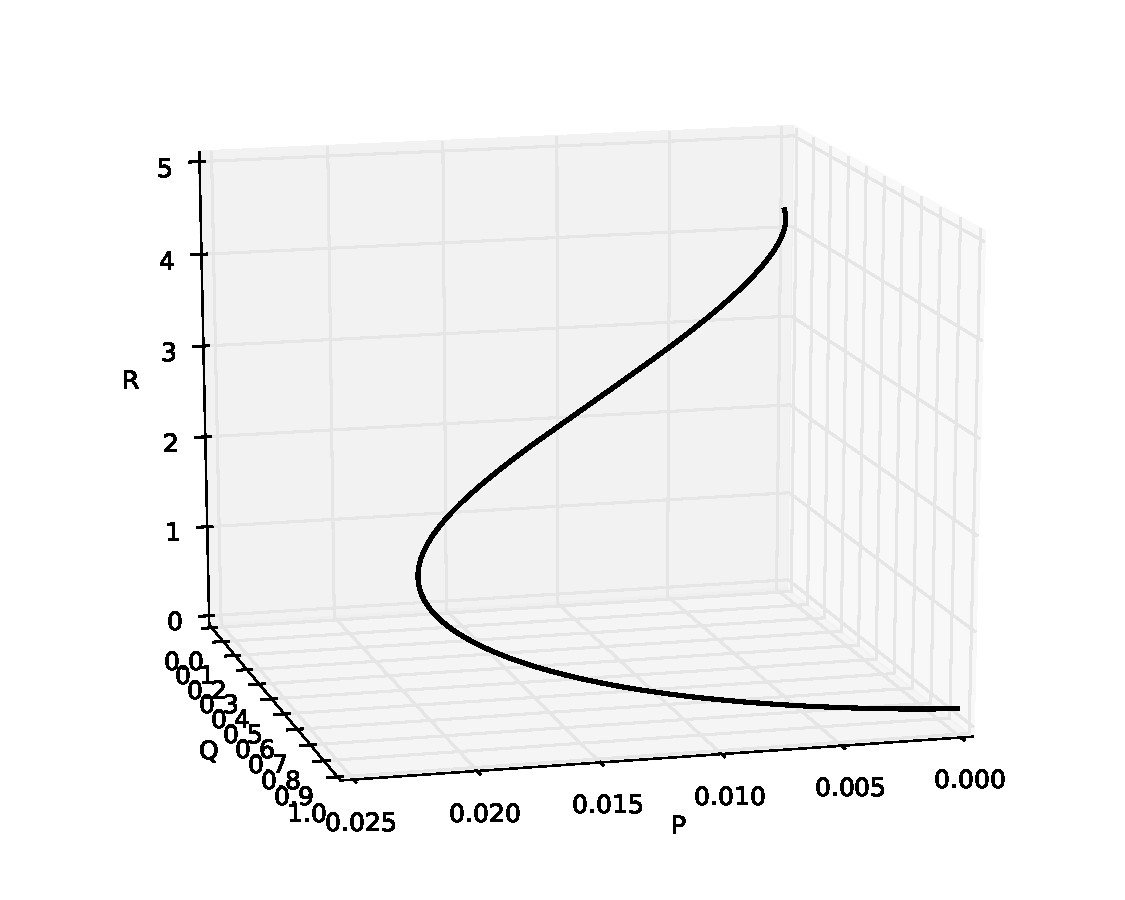
\includegraphics[width=6cm]{heteroPQR.pdf}\label{fig:temperature}
  }
  \quad \quad
  \subfigure[strain]{
  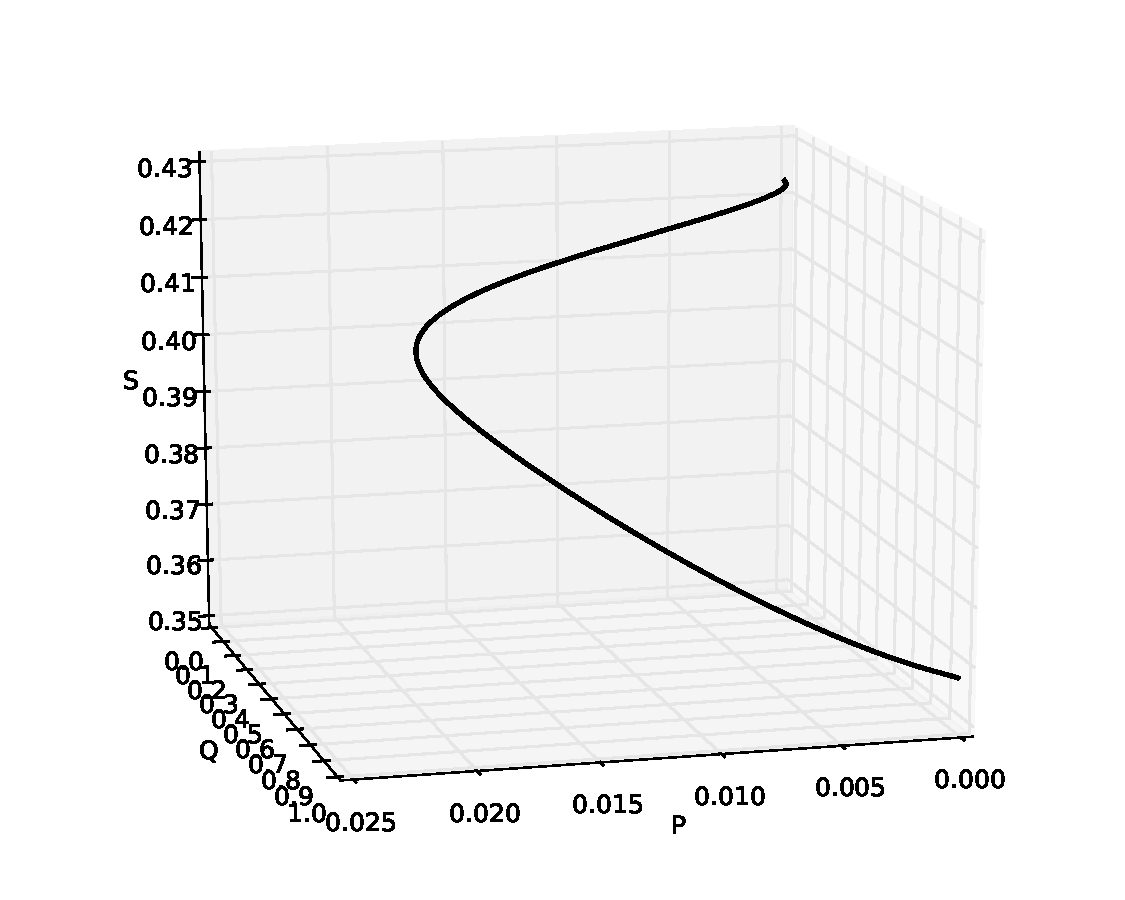
\includegraphics[width=6cm]{heteroPQS.pdf}\label{fig:strain}
  }
  \subfigure[strain-rate]{
  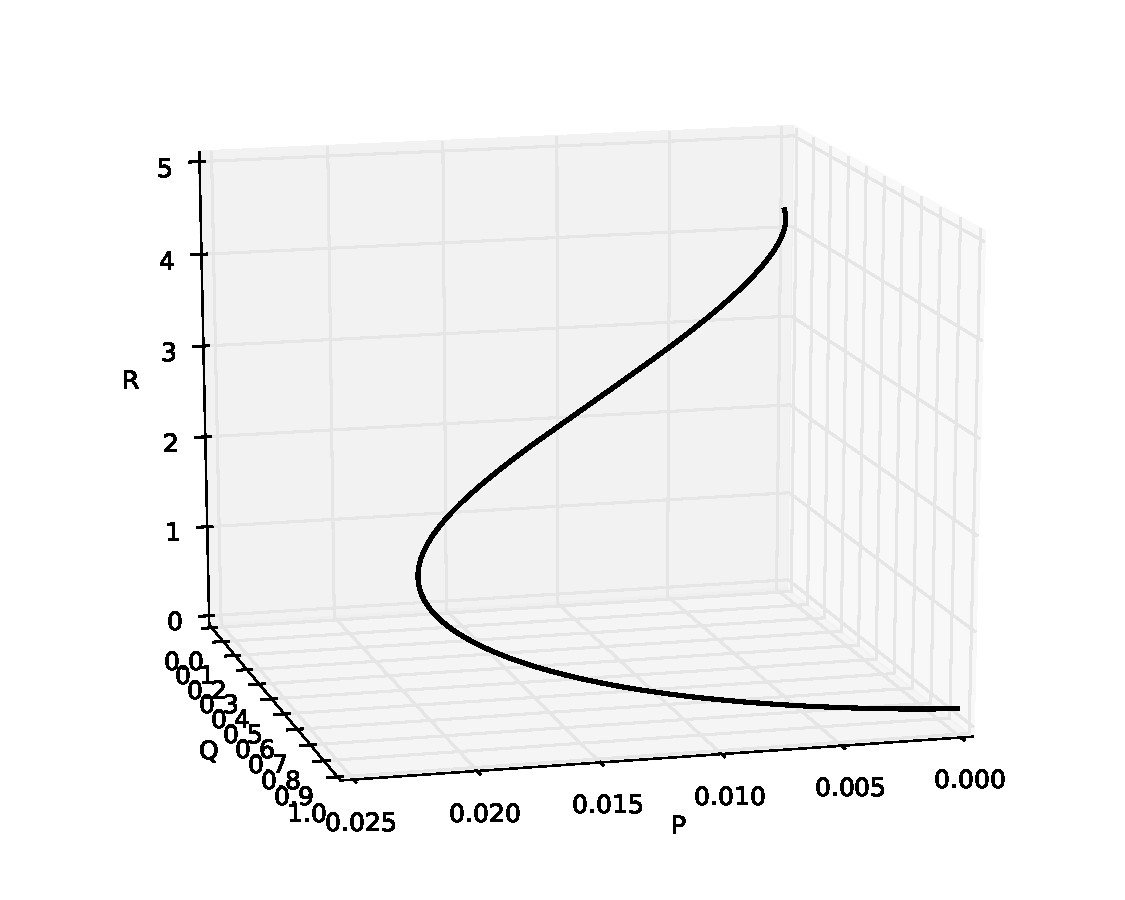
\includegraphics[width=6cm]{heteroPQR.pdf}\label{fig:strain rate}
  }
  \quad \quad
  \subfigure[velocity]{
  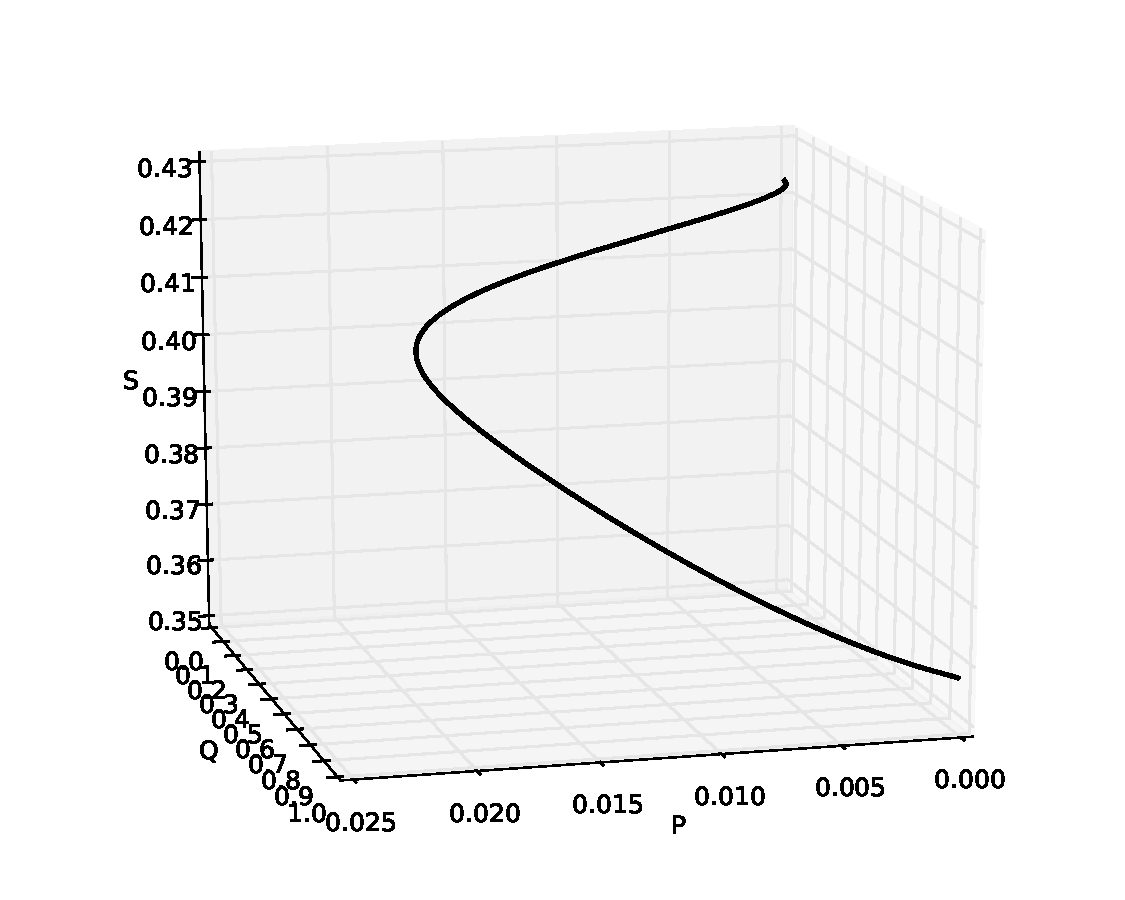
\includegraphics[width=6cm]{heteroPQS.pdf}\label{fig:velocity}
  }
  \subfigure[stress]{
  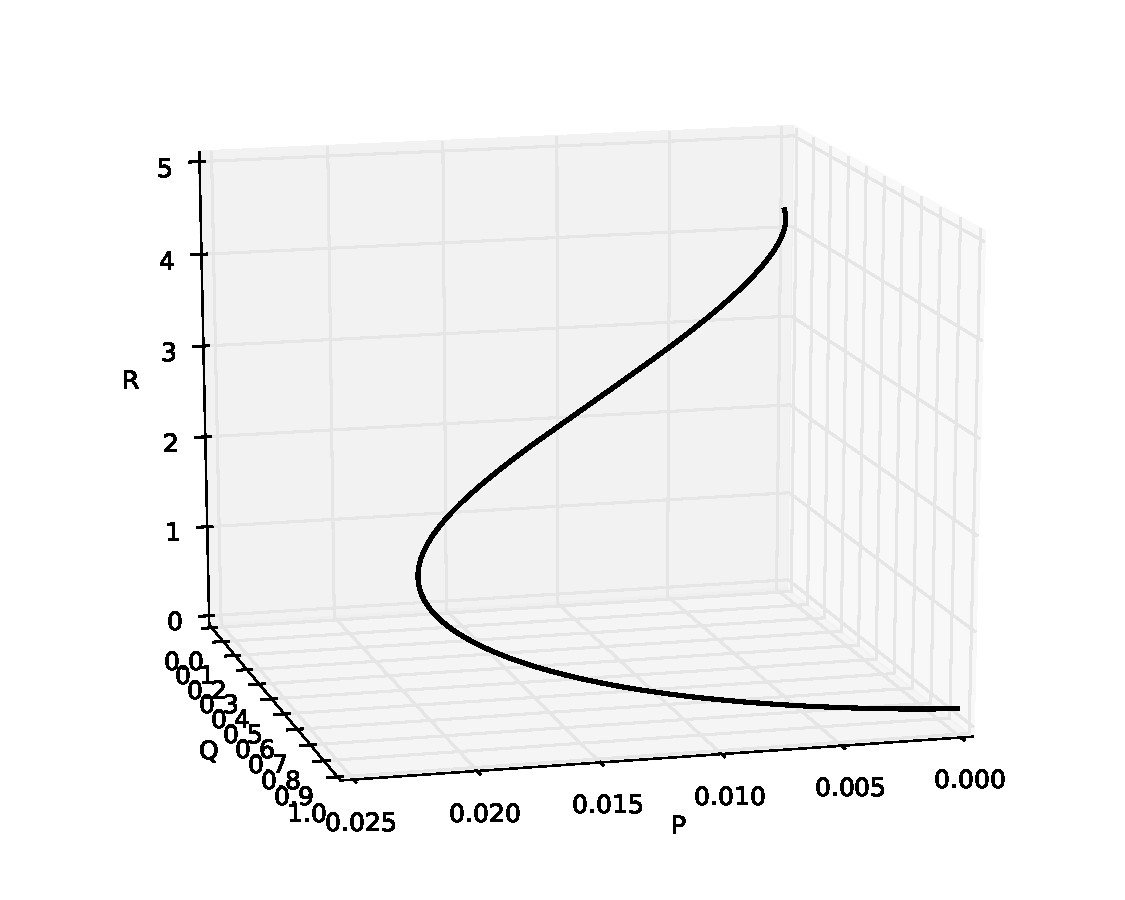
\includegraphics[width=6cm]{heteroPQR.pdf}\label{fig:stress}
  }
  \caption{{\red Physical variables. pdf files to be replaced!}} \label{fig:physical}
\end{figure}

\pagebreak

\begin{figure}[ht]
 \centering
  \subfigure[First \texttt{AUTO} continuation]{
  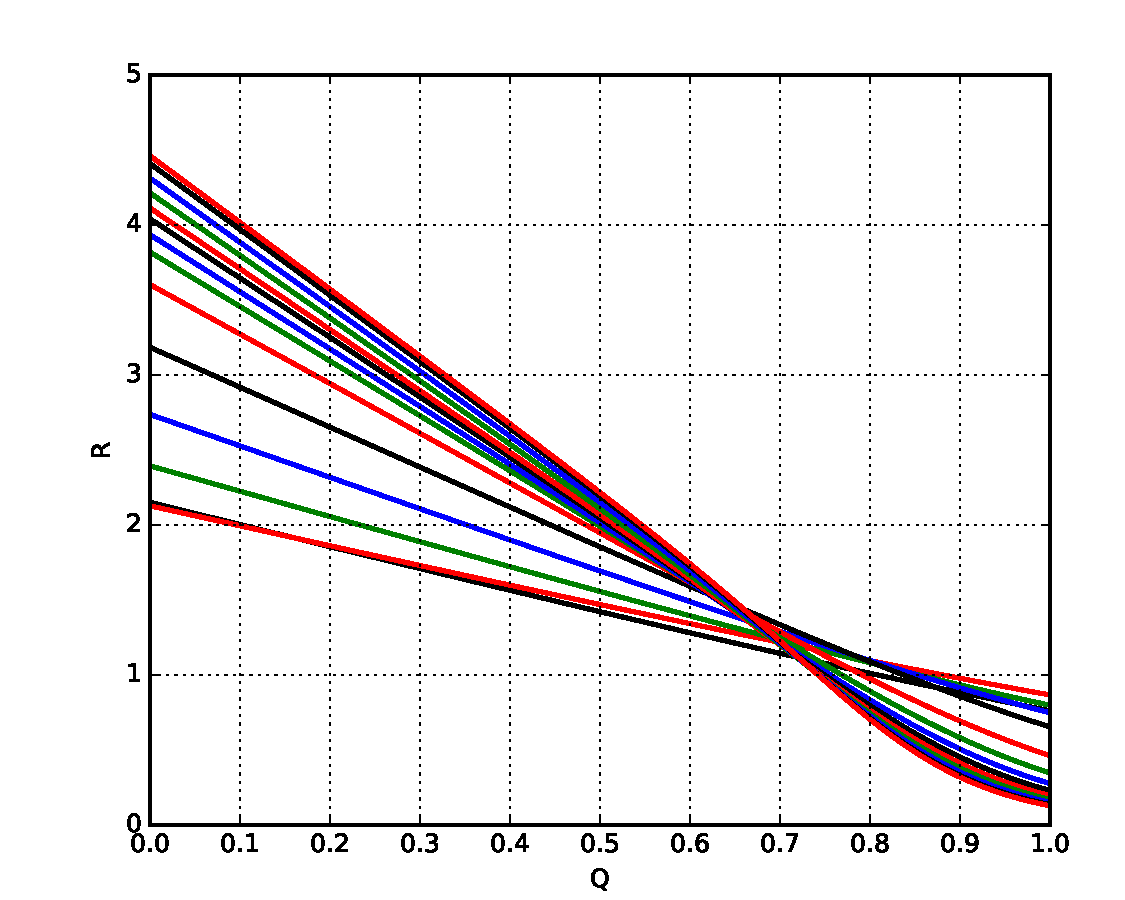
\includegraphics[width=6cm]{firstrun.pdf}\label{fig:run1}
  }
  \quad \quad
  \subfigure[Second \texttt{AUTO} continuation]{
  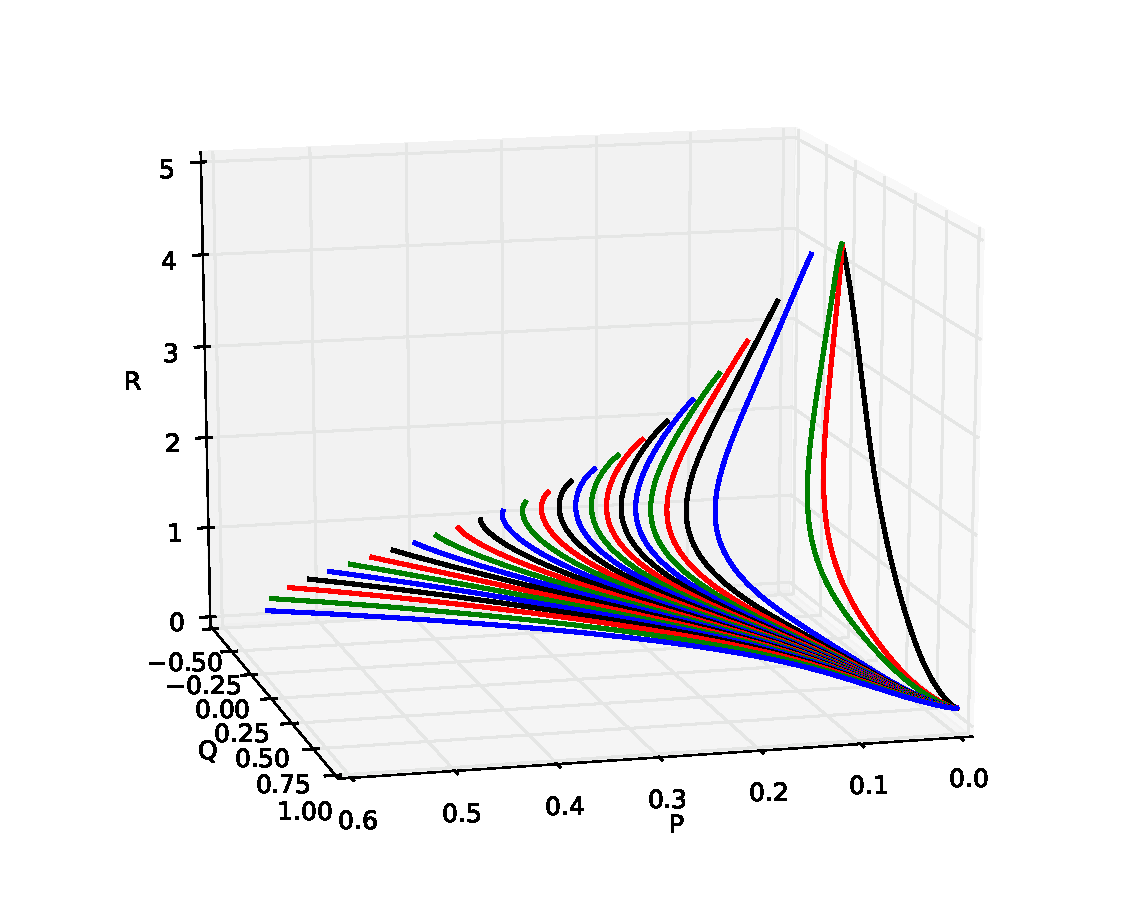
\includegraphics[width=6cm]{secondrun.pdf}\label{fig:run2}
  }
  \caption{caption} \label{fig:run12}
\end{figure}

\begin{figure}[ht]
 \centering
  \subfigure[$pqr$-space]{
  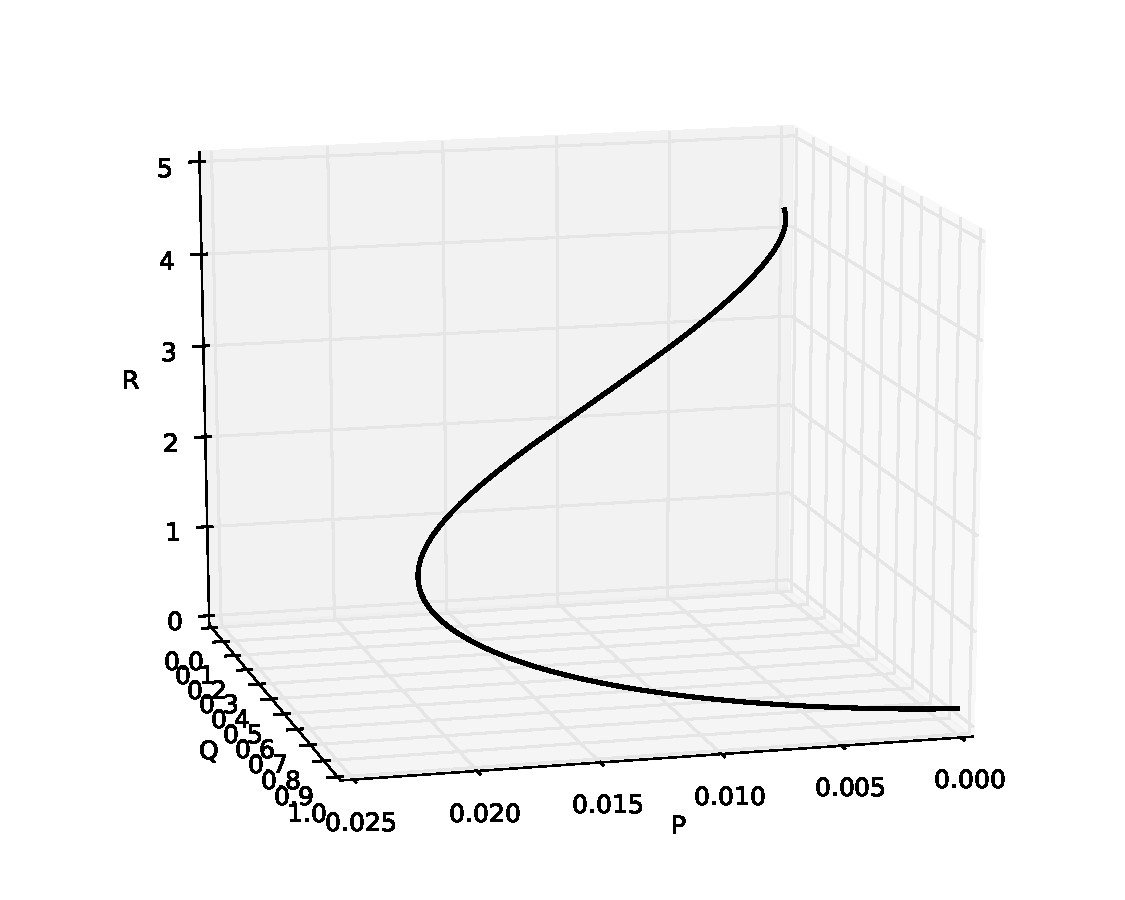
\includegraphics[width=6cm]{heteroPQR.pdf}\label{fig:PQR}
  }
  \quad \quad
  \subfigure[$pqs$-space]{
  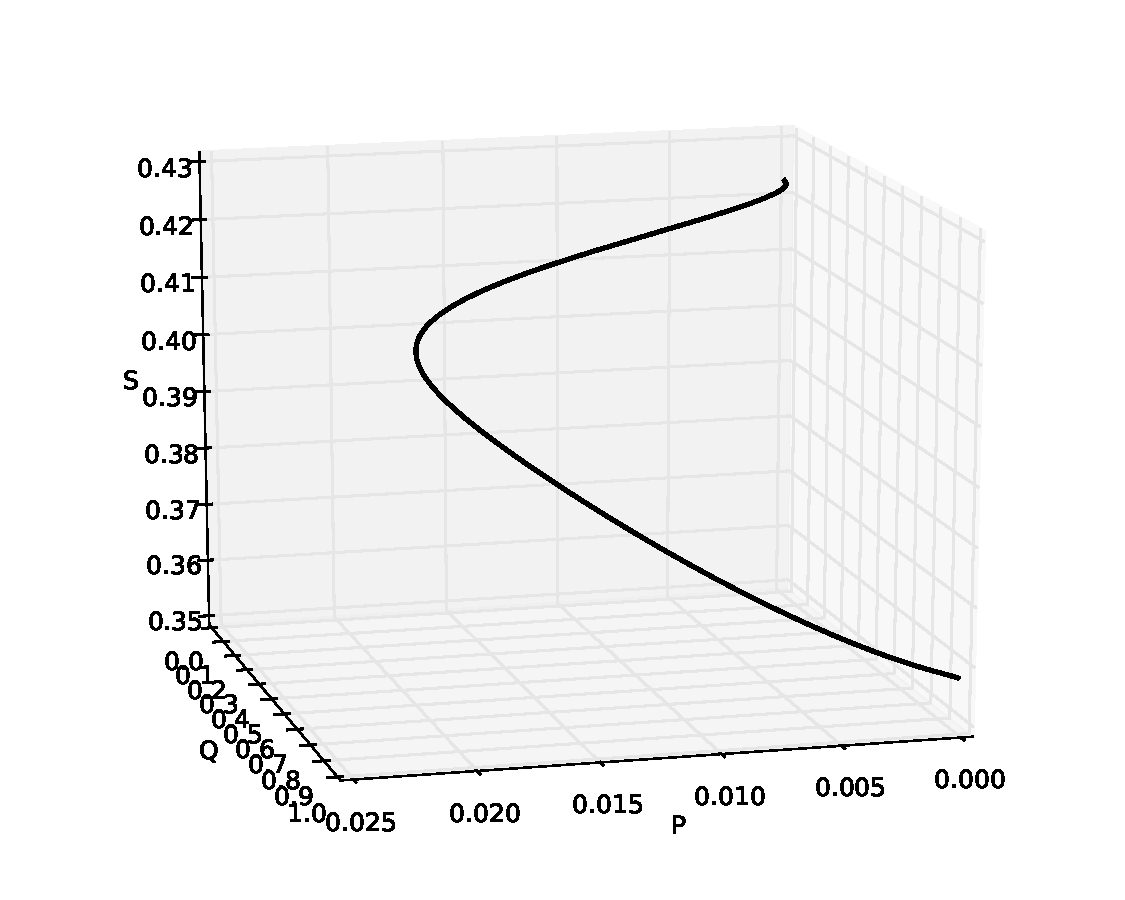
\includegraphics[width=6cm]{heteroPQS.pdf}\label{fig:PQS}
  }
  \caption{Heteroclinic orbit captured by \texttt{AUTO} at $(\alpha,m,n,\lambda) = (7.663,2.584,0.100,2.323)$} \label{fig:hetero}
\end{figure}



To summarize the goal of this section, we aim to capture the single heteroclinic orbit curve that emanates from $M_0$ in the direction of $X_{01}$ and is attracted to $M_1$. It exists as a curve on 2-surface of $W^u(M_0)\cap W^s(M_1)$, the intersection of two 3-dimensional manifolds in $\mathbb{R}^4$. The difficulty lies in that both of $M_0$ and $M_1$ are saddle points: The numerical time integration in both forward and backward time direction suffers the instability due to the extra unstable dimension.

The method of continuation developed in {(Doedle, Friedman)} was successfully applied on our objective.

In the below, we demonstrate the procedure for the characterization of the heteroclinic.
\subsection{Continuation by AUTO}
{\bf \noindent Step 1}
The system when $\alpha=0$ is especial that the equations for $p$, $q$, and $r$ decouples from that for $s$. The reduced system carries only the three dimensional unstable manifold of $M_0$, characterizing the heteroclinic orbit a node-saddle connection. In principle, by running time backward and shooting the orbit in the small neighborhood of $M_1$, any heteroclinic orbit can be computed as accurate as the numerical time integrator allows. Even more exact preparation has been carried out. The plane $p\equiv0$ is especial that the equation $q$ decouples from the rest. The following 1-parameter family of explicit solutions precisely specifies one curve on the plane. These explicit formulas are available when $n= \frac{1}{k}$, $k$ integer.
\begin{align}
 p&\equiv0, \quad q(t) = \frac{1}{1+C_1e^{-t}},\\
 r(t) &= \frac{r_0 \left(C_1 + e^t\right)^k}{ \displaystyle \sum_{j=0}^k \frac{kW_0}{kW_0 -j}\begin{pmatrix} k\\j\end{pmatrix}C_1^{k-j} e^{jt}} , \quad \text{where $W_0= - \frac{(m+n)r_0}{\lambda}$}.
\end{align}
$C_1$ accounts for the time translation factor and we pick $C_1=1$.

{\bf \noindent Step 2}
In the step 2, we integrate $s$ by numerical time integrator in $[-10,10]$. The timespan was so chosen for $(p,q,r,s)|_{t=\pm10}$ respectively falls into the point within our tolerance of closeness to $M_0$ and $M_1$. The starting point of shooting is $(p,q,r,s)|_{t=-10} = M_0 + \epsilon_0 \nu_0$, $\nu_0 = X_{02}$, meaning that the distance from $M_0$ is $\epsilon_0$ and the orbit is on the $p\equiv0$ plane. Having those fixed, the following non-autonomous equation is integrated from $-10$ to $10$.
$$\dot{s} =s\Big(\frac{-m-n}{\lambda}(r(t)-a) + \lambda p(t)r(t) + q(t) - \frac{1}{\lambda}r(t)\big(s- (1+m+n)\big) - \frac{n}{\lambda}\Big).$$

After calculation, at the finial point $(p,q,r,s)|_{t=10}$, we project the vector $(p,q,r,s)|_{t=10}- M_1$ to the stable {\it subspace} of $M_1$, where we can explicitly calculate $\epsilon_1$ and $\nu_1 \in \underset{}{ \textrm{Span}}\{X_{11},X_{12},X_{14}\}$, $|\nu_1|=1$ such that
$\pi\big((p,q,r,s)|_{t=10}- M_1\big) =\epsilon_1 \nu_1$.

At this stage, the data $(p,q,r,s)(t)$ for a fixed orbit, which is for $\alpha=0$ and is on the $p\equiv0$ plane,  $t\in[-10,10]$ at $t_i$, $i=0,\cdots,N$ grid points are at gsdgdf ready. This can be prepared as accurate as the numerical time integrator allows.

{\bf \noindent Step 3}
We run \texttt{AUTO} that starts off from the above prepared data. In this first run, we keep $\nu_0$ fixed but allowing $\alpha$, $m$, $\lambda$, $\epsilon_0$, $\epsilon_1$, $\nu_1$ continued.  The goal is to let \texttt{AUTO} capture the orbit that is still on $p\equiv0$ plane but with $\alpha$ not anymore trivial.

{\bf \noindent Step 4}
Among orbits captured in the Step 3, we pick one and conduct the second \texttt{AUTO} run from it. Importantly, we keep now $\alpha$, $m$, $\lambda$, $n$ fixed but vary $\nu_0$ in $\underset{}{ \textrm{Span}}\{X_{01},X_{02},X_{03}\}$. The goal is to capture {\it the heteroclinic orbit} with $\nu_0=X_{01}$. By this run, we are capturing the 2-surface of the heteroclinic orbits that is $W^u(M_0)\cap W^s(M_1)$. \texttt{AUTO} not only was able to capture as many heteroclinics on the 2-surface as we demanded but to capture the heteroclinic with $\nu_0$ practically coincides with $X_{01}$.

{\red
To Do :

1. workout introduction

1. workout section 4

1. continuation method explanation in section 5

1. add paragraphs on $n=0$ case phase space analysis in section 4

1. streamline the Appendix

1. workout the bibliography

1. proofreading

}





\pagebreak
\appendix
% \section*{Appendix}
\renewcommand\thetheorem{\Alph{theorem}}
\newcounter{tmp}
\setcounter{theorem}{\thetmp}
\section{Analyticity of a simple root of a polynomial}



\begin{theorem}{\cite[p. 24]{L1966}} \label{thm:anal} Let $f_j(w,z)$, $j=1,\cdots,m$, be analytic functions of $(w,z)=(w_1,\cdots,w_m,z_1,\cdots,z_n)$ in a neighborhood of a point $(w^0,z^0)$ in $\mathbb{C}^m\times \mathbb{C}^n$, and assume that $f_j(w^0,z^0)=0$, $j=1,\cdots,m$ and that
$$ \det\Big( \frac{\partial f_j}{\partial w_k} \Big)_{j,k=1}^m \ne 0 \quad \text{at $(w^0,z^0)$}.$$
Then the equations $f_j(w,z)=0$, $j=1,\cdots,m$ have a uniquely determined analytic solution $w(z)$ in a neighborhood of $z_0$, such that $w(z^0)=w^0$.
\end{theorem}

\section{Index conditions of Coddington-Levinson} \label{sec:Index}

In the below, we check the index condition of the Coddington-Levinson.

\noindent{\bf subcase 1 $q=-\alpha+m+n>0$:} The real parts of eigenvalues are all negative for large $\tau$. Suppose \eqref{eq:auxquad} has two negative real roots so that  $-n\l^2 + \frac{1}{\tau}\lambda_3'(0)<\frac{1}{\tau}z_2(0)<\frac{1}{\tau}z_1(0)<0$, for large $\tau<\infty$.  Then we can check for instance
$\displaystyle\int_{\tau_1}^{\tau_2} (z_1(0)-z_1(0))\frac{1}{s} \; ds = 0< 1$,
or $1\in I_2$ for the fixed index $1$. $K=1$ is used in the computation. On the other hand,
$$ \lim_{\tau \rightarrow \infty}\int_{\tau_0}^\tau (z_1(0)-z_2(0))\frac{1}{s} \; ds = \infty, \quad  \int_{\tau_1}^{\tau_2} Re (z_1(0)-z_2(0))\frac{1}{s} \; ds > -1,$$
or $2\in I_1$ for the fixed index $1$ and
$$ \lim_{\tau \rightarrow \infty}\int_{\tau_0}^\tau (z_1(0)-\lambda_3'(0))\frac{1}{s} + n\l^2 \; ds =\infty, \quad  \int_{\tau_1}^{\tau_2} (z_1(0)-\lambda_3'(0))\frac{1}{s} + n\l^2 \; ds > -1,$$
or $3\in I_1$ for the fixed index $1$.

 Similarly we can proceed to check the index condition for all other cases, with $K=1$.
%For $2$ fixed, on the other hand, $\displaystyle\int_{t_1}^{t_2} Re (z_2(0)-z_1(0))\frac{1}{s} \; ds < 1$, or $1\in I_2$.
We summarized the result in the below. In all cases in the below $K=1$ is enough as were in the examples.
\begin{align*}
  \text{Fix $\ell=1$:}&& 2,3&\in I_1, & 1&\in I_2\\
  \text{Fix $\ell=2$:}&& 3&\in I_1, & 1,2&\in I_2\\
  \text{Fix $\ell=3$:}&& & & 1,2,3&\in I_2.
\end{align*}
Now, when \eqref{eq:auxquad} has two complex roots with negative real parts so that $-n\l^2 + \frac{1}{\tau}\lambda_3'(0)<Re\Big(\frac{1}{\tau}z_2(0)\Big)=Re\Big(\frac{1}{\tau}z_1(0)\Big)<0$ for large $\tau<\infty$, the results are
\begin{align*}
  \text{Fix $\ell=1$:}&& 3&\in I_1, & 1,2&\in I_2,\\
  \text{Fix $\ell=2$:}&& 3&\in I_1, & 1,2&\in I_2,\\
  \text{Fix $\ell=3$:}&& & & 1,2,3&\in I_2.
\end{align*}


\noindent{\bf subcase 2 $q=-\alpha+m+n=0$:} In this case, the roots of \eqref{eq:auxquad} are
$$ z_1(0)=0, \quad z_2(0) = -\frac{1+m+\alpha}{1+m}$$
and the sign of $z_1(\epsilon)$ is determined by the next order term. Nevertheless we have
$-n\l^2 + \frac{1}{\tau}\lambda_3'(0)<\frac{1}{\tau}z_2(0)<0=\frac{1}{\tau}z_1(0)$ for large $\tau<\infty$ and
\begin{align*}
  \text{Fix $\ell=1$:}&& 2,3&\in I_1, & 1&\in I_2\\
  \text{Fix $\ell=2$:}&& 3&\in I_1, & 1,2&\in I_2\\
  \text{Fix $\ell=3$:}&& & & 1,2,3&\in I_2.
\end{align*}

\noindent{\bf subcase 3 $q=-\alpha+m+n<0$:}
The characteristic polynomial has precisely one positive real root and two negative real roots. If we label them so that
$-n\l^2 + \frac{1}{\tau}\lambda_3'(0)<\frac{1}{\tau}z_2(0)<0<\frac{1}{\tau}z_1(0)$, for large $\tau<\infty$ then
\begin{align*}
  \text{Fix $\ell=1$:}&& 2,3&\in I_1, & 1&\in I_2\\
  \text{Fix $\ell=2$:}&& 3&\in I_1, & 1,2&\in I_2\\
  \text{Fix $\ell=3$:}&& & & 1,2,3&\in I_2.
\end{align*}

\section{Stability analysis of a non-autonomous system}
We study the stability of a linear non-autonomous system
$$ x'=A(t) x.$$%, \quad A(t) \rightarrow A_\infty \quad \text{as $t \rightarrow \infty$}.$$
The entries $A_{ij}(t)$, $i,j=1,\cdots,d$ are assumed to be bounded. As the vector field is Lipschitz in $x$, it admits the semi-group $F(t)$ (in fact a group for all $t$) characterized by the property $y(t)=F(t)y(0)$. When it is a system of non-autonomous equations, due to the coupling, the maximum of the real parts of the eigenvalues does not necessarily accounts for the operator norm of $F(t)$; $A(t)$ with negative eigenvalues can results in having an exponentially growing solution, showing $\|F(t)\|$ exponentially grows.

On the contrary, like for diagonal matrices, $\|F(t)\|$ can be read off from $A(t)$ when the coupling is in an appropriate sense weaker. $A(t)$ can be by similarity transform turned into the form that has less coupling such as diagonal or Jordan normal form. The price is an additional term due to that the decomposition is also time dependent. More precisely, If $A(t) = P(t)U(t)P(t)^{-1}$, and if $y\triangleq P(t)^{-1}x$ then $y$ satisfies the system
\begin{equation} y' = U(t)y - P(t)^{-1}P'(t)y. \label{eq:after_fact} \end{equation}

Assuming the operator norm of the solution map $F(t)$ associated to $U(t)$ is computable, we look if the coupling by the remainder term is negligible. Following proposition sheds light on which cases are feasible ones.
\begin{proposition} \label{prop:stab}
 Suppose
 \begin{equation}
x' = U(t)x + \mathcal{E}(t)x, \label{eq:x}
 \end{equation}
where $U_{ij}(t)$ are bounded and the associated solution map $F(t)$ has the norm $\|F\|(t) \le h(t)=\exp\left(\int_0^t \theta(s)\; ds\right)$ for some $\theta(t)$. Assume that $\mathcal{E}_{ij}(t)$ decay as $t \rightarrow \infty$ so that they are integrable, i.e.,
 $$ \int_{a_0}^\infty |\mathcal{E}_{ij}(s)| \; ds < \infty, \quad \forall i,j=1,\cdots,d \quad \text{for some $a_0$.}$$
 Then, for some $a$ every solution $\|x\|_{L^\infty[a,t]} \le 2h(t)$. Furthermore, if $y(t)=F(t)y(0)$ is the one attains the operator norm, i.e.,
 $$ \lim_{t \rightarrow \infty}\frac{y(t)}{\|F\|(t)} = y_\infty \quad \text{nontrivial,}$$
 there is a solution $x(t)$ of \eqref{eq:x} such that $\displaystyle \frac{2}{3}\frac{\|y(t)\|_{L^\infty[a,t]}}{\|F\|(t)}\le\frac{\|x(t)\|_{L^\infty[a,t]}}{\|F\|(t)} \le 2\frac{\|y(t)\|_{L^\infty[a,t]}}{\|F\|(t)}.$
\end{proposition}
\begin{proof}
%  Without loss, we may set $h(t) = \exp\left(\int_0^t \theta(s)\; ds\right)$ by setting $\theta(t) = \log(h(t))'$.
We rewrite \eqref{eq:x} in the form
 \begin{align*}
  x' - \theta(t)x &= \big(U(t)-\theta(t)\big)x + \mathcal{E}x \quad \text{or}\\
  \xi' &=\big(U(t)-\theta(t)\big)\xi + \mathcal{E}\xi, \quad \text{where $\xi\triangleq \exp\left(-\int_0^t \theta(s)\; ds\right) x$}.
 \end{align*}
 Let $G(t)$ be the solution map associated to $U(t)-\theta(t)$. Since $F(t)x(0)=x(t)$ \\$= \exp\left(\int_0^t \theta(s)\; ds\right)\xi(t)= \exp\left(\int_0^t \theta(s)\; ds\right)G(t)\xi(0)=\exp\left(\int_0^t \theta(s)\; ds\right)G(t)x(0)$, for all $x(0)\in \mathbb{R}^d$, $G(t) = F(t)\exp\left(-\int_0^t \theta(s)\; ds\right)$ and $\|G\|(t)\le 1$. Using $G(t)$ we further write
 $$ \xi(t) = G(t-a)\xi(a) + \int_a^t G(t-\tau)\mathcal{E}(\tau)\xi(\tau) \; d\tau \quad \text{for some $a$ we choose later.}$$
 Note that if $\bar\xi$ is a bounded function then the the expression right-hand-side well-defines an operator $S:L^\infty([a,\infty)) \mapsto L^\infty([a,\infty))$ because $t\ge \tau\ge a$, $G$ is bounded and $\mathcal{E}$ is integrable. $S\bar\xi$ has the same initial value $\xi(a)$. If $a$ is chosen so large that $\int_a^\infty \|G\| \; |\mathcal{E}_{ij}|\; d\tau < \frac{1}{2}$ then this is a contraction mapping. Therefore solution exists with the initial value $\xi(a)$. Since $\xi(a)$ was arbitrary, every independent solution is attained.
 From the integral representation of $\xi(t)$, we have
 \begin{align*}
 \|\xi(t)\|_{L^\infty([a,t])} &\le \|G(t-a)\xi(a)\|_{L^\infty([a,t])} + \left\|\int_a^t G(t-\tau)\mathcal{E}(\tau)\xi(\tau) \; d\tau\right\|_{L^\infty([a,t])} \\
 &\le \|G(t-a)\xi(a)\|_{L^\infty([a,t])} + \frac{1}{2} \|\xi(t)\|_{L^\infty([a,t])},\\
 \|\xi(t)\|_{L^\infty([a,t])} &\le 2 \|G(t-a)\xi(a)\|_{L^\infty([a,t])} \le 2\sup_t \|G\|(t) \le 2.
 \end{align*}
 This gives the boundedness of the solution. Now, let $\xi(t)$ and $\xi(a)$ be that its semi-group part is the $y(t)$ grows as same as the operator norm does. The second assertion follows from
 \begin{align*}
&\big\|\xi(t) - G(t-a)\xi(a)\big\|_{L^\infty([a,t])} = \left\|\int_a^t G(t-\tau)\mathcal{E}(\tau)\xi(\tau) \; d\tau\right\|_{L^\infty([a,t])} \le \frac{1}{2} \|\xi(t)\|_{L^\infty([a,t])},\\
&\big\|G(t-a)\xi(a)\big\|_{L^\infty([a,t])} \le \big\|\xi(t) - G(t-a)\xi(a)\big\|_{L^\infty([a,t])} + \big\|\xi(t)\big\|_{L^\infty([a,t])} \le \frac{3}{2} \|\xi(t)\|_{L^\infty([a,t])}.
 \end{align*}
\end{proof}
\begin{remark}
 \begin{enumerate}
  \item Proposition \ref{prop:stab} does not assume a special structure of $U(t)$ but assumes its associated $\|F\|(t)$ has estimated, no matter what couplings take place. Given the estimate, it persists under the perturbation by $\mathcal{E}$, whose entries are integrable. Moreover, the largest growth of the perturbed system is precisely as same as unperturbed one.
  \item The condition that the $\mathcal{E}_{ij}(t)$ is integrable cannot be relaxed. $x=t$ of  $x'=\frac{x}{t}$, is an example in which the asymptotic stability fails by the contribution of the non-integrable coefficient.
 \end{enumerate}
\end{remark}

It remains how we can estimate $\|F\|(t)$ that is associated with $U(t)$. For completeness, we next provide an estimate of $\|F\|(t)$ associated to an upper triangular matrix. This is extended to a $U(t)$ that is block diagonal with upper triangular blocks because the solution map $F(t)$ is then decoupled as well block-wisely.

 \begin{proposition}[stability of triangular matrix] \label{prop:tri-stab}
 Suppose $y' = U(t) y$ and $U(t)$ be an upper triangular matrix with bounded entries. Suppose that there is a function $\theta(t)$ and a constant $A$ such that for all diagonal entries $\lambda_i(t)$,
 \begin{align} \label{eq:stabcond}
%   &\lim_{t \rightarrow \infty} t^{-d} \int_0^t \theta(s)- Re\lambda_i(s)\; ds \rightarrow \infty,\\
  &\int_{t_1}^{t_2} \theta(s)-Re\lambda_i(s)\; ds > -A \quad \text{whenever $0\le t_1 \le t_2$.}
 \end{align}
 Then for $i=1,\cdots,d$
 \begin{equation} \label{eq:triestim}
|y_{i}(t)| \le C\big( 1 + t + \cdots + t^{d-i}\big) \exp\left( \int_0^t \theta(s)\;ds\right)% \rightarrow 0 \quad \text{as $t \rightarrow \infty$.}
 \end{equation}
\end{proposition}
\begin{proof}
 We prove the assertion by induction in the descending order. For $i=d$, $y_d(t)=y_d(0)\exp\left( \int_0^t \lambda_d(s)\;ds\right)=y_d(0)\exp\left( \int_0^t \theta(s)-\theta(s)+\lambda_d(s)\;ds\right)$ and thus $|y_d(t)| \le Ce^A\exp\left( \int_0^t \theta(s)\;ds\right)$ by \eqref{eq:stabcond}. Now, if the statement holds for $i$, we see that
 \begin{align*}
  y_{i-1}' -\lambda_{i-1}y_{i-1} = \sum_{j\ge i} U_{i-1,j}(t)y_j(t) = g(t)
 \end{align*}
 and $|g(t)| \le C\big( 1 + t + \cdots + t^{d-i}\big) \exp\left( \int_0^t \theta(s)\;ds\right)$ for some another constant $C$ because $U_{ij}(t)$ are bounded. Therefore
 \begin{align*}
  y_{i-1}(t) &= \exp\left( \int_0^t \lambda_{i-1}(s)\;ds\right) \left(y_{i-1}(0) + \int_0^t \exp\left( \int_0^\tau -\lambda_{i-1}(s)\;ds\right)g(\tau) \; d\tau\right)\\
  &=\exp\left( \int_0^t \theta(s)-\theta(s)+\lambda_{i-1}(s)\;ds\right) y_{i-1}(0) \\
  &+ \exp\left( \int_0^t \theta(s)\;ds\right)\underbrace{\int_0^t \exp\left( \int_\tau^t \lambda_{i-1}(s)-\theta(s)\;ds\right)g(\tau)\exp\left( -\int_0^\tau \theta(s)\;ds\right) \; d\tau}_{\triangleq \varphi(t)}
  \end{align*}
 Note that $\varphi(0)=0$ and $|\varphi'(t)| = \left|g(t)\exp\left( \int_0^t -\theta(s)\;ds\right)\right|\le C\big( 1 + t + \cdots + t^{d-i}\big)$ by the assumptions. Thus $|\varphi(t)|\le C\big( 1 + t + \cdots + t^{d-i+1}\big)$ for some another constant $C$. Therefore
 $$|y_{i-1}(t)| \le C\big( 1 + t + \cdots + t^{d-i+1}\big)\exp\left( \int_0^t \theta(s)\;ds\right).$$
\end{proof}


\begin{remark}
  This estimate shows that the couplings through off-diagonal terms does spoil the asymptotic stability when the eigenvalues decay to $0$ as $t \rightarrow \infty$ but not so much to be integrable. Suppose that every eigenvalue has negative real parts bounded by $\theta(t) = -\frac{k}{t}$ for some $k$. Then the estimate \eqref{eq:triestim} fails to guarantee the asymptotic stability unless otherwise $k\ge d$ because $\exp\left( \int_1^t \theta(s)\;ds\right) =\exp\left( -\int_1^t \frac{k}{s}\;ds\right) =t^{-k}.$ This is the typical behavior of the Jordan block.
\end{remark}

Lastly, the case where $U(t)$ is diagonal is considered. In this case, not only the explicit formula of the solution map $F(t) = \textrm{diag}\left[ \exp\left(\int_0^t \lambda_i(s)\; ds\right) \right]$ is available but also it is possible to spot every modes. Indeed, the unperturbed system is totally decoupled so that every mode remains unmixed and survives. This property is in fact shared by the upper triangular matrix; this can be seen by just taking $\hat{\ell}$ the coordinate basis as an initial data. The next Coddington-Levinson theorem shows that for a diagonal matrix, under the suitable spectral gap conditions, the ability to discern all modes persists after adding a weak coupling $\mathcal{E}(t)$. The spectral condition is notably precise where the accumulated contribution by non-integrable real parts of eigenvalues matters.

\begin{theorem}{\cite[Diagonal Version]{CL1955}}\label{thm:CL} Let $x(t)\in \mathbb{R}^d$ and $x'(t) = \big(\Lambda(t) + \mathcal{E}(t)\big)x$, where $\Lambda(t)$ is a diagonal matrix with diagonal entries $\lambda_j(t)$, $j=1,\cdots,d$ bounded and $\mathcal{E}(t)$ is a matrix with entries $\mathcal{E}_{ij}$ integrable, i.e., $\int_{a_0}^\infty |\mathcal{E}_{ij}(s)|\; ds < \infty$ $\forall i,j=1,\cdots,d$ for some $a_0$.
Fix an index $\ell$. Suppose we can find the constant $A$ so that either of the following two membership conditions holds for every $i$.

$i \in I_1$ if
\begin{align}
 &\int_{a_0}^\infty Re(\lambda_\ell(s) -\lambda_i(s))\; ds \rightarrow \infty \quad \text{as $t \rightarrow \infty$ for some $a_0$},\label{eq:I1cond1}\\
 &\int_{t_1}^{t_2} Re(\lambda_\ell(s) -\lambda_i(s))\; ds > -A, \quad \text{whenever $t_2\ge t_1\ge 0$} \label{eq:I1cond2}
\end{align}
and $i \in I_2$ if
\begin{align}
 &\int_{t_1}^{t_2} Re(\lambda_\ell(s) -\lambda_i(s))\; ds < A, \quad \text{whenever $t_2\ge t_1\ge 0$}. \label{eq:I2cond}
\end{align}
Then there is an orbit $\varphi_\ell(t)$ $t\ge a$ for some $a$ such that,
\begin{equation}
 \lim_{t \rightarrow \infty} \varphi_\ell(t) \exp\left(-\int_{a}^t \lambda_\ell(s)\; ds\right) = \hat{\ell}, \quad \text{where $\hat{\ell}$ is the $\ell$-th coordinate basis of $\mathbb{R}^d$.}
\end{equation}
\end{theorem}
\begin{proof}
Component-wisely, we can write
\begin{align*}
 \xi_i' & = (\lambda_i-\lambda_\ell)\xi_i + \mathcal{E}_{ij}\xi_j, \quad \text{where $\xi = \exp\left(-\int_a^t \lambda_\ell(s) \; ds\right)x$.}
\end{align*}
We look for a solution of the integral representation
\begin{align*}
 \xi_i(t) &= \hat\ell_i + \int_a^t \exp\left(\int_\tau^t \lambda_i(s)-\lambda_\ell(s) \; ds\right)\mathcal{E}_{ij}(\tau)\xi(\tau) \; d\tau && \text{if $i\in I_1$,}\\
% \end{align*}
% if $i\in I_1$, where $\hat{\ell}_i = \delta_{\ell i}$ of Kronecker delta and
% \begin{align*}
 \xi_i(t) &= \hat\ell_i -\int_t^\infty \exp\left(\int_t^\tau -\lambda_i(s)+\lambda_\ell(s) \; ds\right)\mathcal{E}_{ij}(\tau)\xi(\tau) \; d\tau && \text{if $i\in I_2$,}
\end{align*}
where $\hat{\ell}_i = \delta_{\ell i}$ of Kronecker delta. Let $t\ge a$ so large that $e^A\int_a^\infty |\mathcal{E}_{ij}(\tau)|\; d\tau < \frac{1}{2}$. Then by \eqref{eq:I1cond2} and \eqref{eq:I2cond}, for given $\bar\xi(t)$ bounded $t\ge a$, the expression right-hand-side defines an operator $S$ that maps $\bar\xi$ to another bounded function that is defined by the expression. In particular, $\xi=S\bar\xi$ has same initial data $\xi_i(a) = \hat{\ell}_i$ if $i\in I_1$.
% and has same finial data $\displaystyle\lim_{t \rightarrow \infty} \xi_i(t) = \hat{\ell}_i$ if $i\in I_2$.
By the choice of $a$, $\|S\xi - S\bar\xi\|_\infty \le \frac{1}{2}\|\xi-\bar\xi\|_\infty$, $t\ge a$ and thus $S$ is a contraction mapping. The integral equation has the unique solution and $\|\xi_i(t)\|_\infty \le 2$ because the integral is bounded above by $ \frac{1}{2} \|\xi\|_\infty$ and $|\hat{\ell}|=1$.

Now we show that $|\xi(t)-\hat\ell| \rightarrow 0$ as $t \rightarrow \infty$. For given $\epsilon>0$, we show we can choose $t_0$ so large that for $t\ge t_0$, $\big|\xi_i(t)-\hat{\ell}_i\big| \le \epsilon$. If $i\in I_1$, we divide the integral into two parts
\begin{align*}
 &\big|\xi_i(t)-\hat{\ell}_i\big| \le \left|\left\{ \int_a^{t_1} + \int_{t_1}^t \right\} \exp\left(\int_\tau^t \lambda_i(s)-\lambda_\ell(s) \; ds\right)\mathcal{E}_{ij}(\tau)\xi(\tau) \; d\tau \right|.
\end{align*}
By choosing $t_1$ so large the second integral can be made smaller than $ \frac{\epsilon}{2}$ for all $t\ge t_1$. The first integral $$\left|\exp\left(\int_a^t \lambda_i(s)-\lambda_\ell(s) \; ds\right)\int_a^{t_1} \exp\left(\int_a^\tau -\lambda_i(s)+\lambda_\ell(s) \; ds\right)\mathcal{E}_{ij}(\tau)\xi(\tau) \; d\tau \right|$$
can be made smaller than $ \frac{\epsilon}{2}$ because the latter integral in the compact interval $[a, t_1]$ is finite and $\exp\left(\int_a^t \lambda_i(s)-\lambda_\ell(s) \; ds\right) \rightarrow 0$ as $t \rightarrow \infty$ by \eqref{eq:I1cond1}.

If $i\in I_2$, then $\left|\int_t^\infty \exp\left(\int_t^\tau -\lambda_i(s)+\lambda_\ell(s) \; ds\right)\mathcal{E}_{ij}(\tau)\xi(\tau) \; d\tau\right| \rightarrow 0$ as $t \rightarrow \infty$.
\end{proof}

\subsection{Possibility of having absolutely continuous factorization}
As indicated, $U(t)$ is presumed to be in the form we can compute its associated semi-group $F(t)$ while $A(t)$ may not. We have so far discussed the persistence properties of system defined by coefficient $U(t)$, the semi-group part, under the presence of weak coupling $\mathcal{E}(t)$.  Now, we turn our attentions to the continuous factorization of $A(t)$ along with the system \eqref{eq:after_fact}.

All earlier discussions assume the integrability of $|\mathcal{E}_{ij}(t)|$ and this was sharp. In order for the factored system \eqref{eq:after_fact} to be analyzed in this context, the term $-P(t)^{-1}P'(t)$ appeared in \eqref{eq:after_fact} has to decay so fast that the entries are integrable. We look for a factorization where $P'(t)$ decays suitably and $P(t)$ and $P(t)^{-1}$ are absolutely continuous up to infinity.

At best possibility is the diagonalization. If so, then we apply the Theorem by Coddington-Levinson under the spectral gap conditions there. However, not every matrix is diagonalizable and more importantly, this factorization is prone to a perturbation, or we do not in general expect the continuity of the eigenvectors.

At worst possibility is the block Schur factorization, $A(t)=U(t)B(t)U^*(t)$, where $U(t)$ is unitary and $B(t)$ is block upper triangular. This factorization is in general abound and not unique while continuous one can be picked. See [Delci] for the smooth factorization: Under the assumption that the spectrum is partitioned into disjoint sets for all time, the method admits a continuous factorization. What can be said to lie in the middle is a Jordan canonical form. It always exists and is unique up to the permutation of blocks but this factorization lacks the continuity as well. Roughly, better the chance we have for the factorization to be continuous, worse the coupling properties we obtain.


\cite{L1966}
% {\red
% In the below, we provide the result again by Coddington and Levinson on a sufficient condition to have absolutely continuous eigenvectors.
% \begin{proposition}
%  Assumption. Then $A(t) = P(t)\Lambda(t)P(t)^{-1}$
% \end{proposition}
% }


\begin{thebibliography}{10}

\bibitem{L1966}
{\sc H\"ormander, Lars},
{\it An introduction to complex analysis in several variables},
(D. Van Nostrand Co., Inc., Princeton, N.J.-Toronto, Ont.-London (1966).

\bibitem{CL1955}
{\sc Coddington, Earl A. and Levinson, Norman},
{\it Theory of ordinary differential equations},
(McGraw-Hill Book Company, Inc., New York-Toronto-London 1955).



\tcr{ References from IMA paper}


\bibitem{BKT}
{\sc Th. Baxevanis, Th. Katsaounis and A.E. Tzavaras},
{\sl Adaptive finite element computations of shear band formation}
Math. Models Meth. Appl. Sciences, (2010), in press.


\bibitem{BPV}
{\sc M.Bertsch, L.A.Peletier and S.M.Verduyn Lunel},
{\sl The effect of temperature dependent viscosity on shear flow of incompressible fluids}
\newblock SIAM J. Math. Anal., {\bf 22} (1991), 328-343.


\bibitem{CDHS}
{\sc R.J.Clifton, J.Duffy, K.A.Hartley and T.G.Shawki},
{\sl On critical conditions for shear band formation at high strain rates}, Scripta Met., {\bf 18} (1984), pp. 443-448.

\bibitem{CCHD}
{\sc L.S.Costin, E.E.Crisman, R.H.Hawley, and J.Duffy},
{\sl On the localization of plastic flow in mild steel tubes under dynamic torsional loading}
 In "Proc. 2nd Conf. on the Mechanical Properties of Materials at high rates of strain",
 Inst. Phys. Conf. Ser. no 47, Oxford, 90, 1979.

\bibitem{DH}
{\sc C.M.Dafermos and L.Hsiao},
{\sl Adiabatic shearing of incompressible fluids with temperature dependent viscosity}
Quart. Appl. Math., {\bf 41} (1983), 45 - 58.


\bibitem{DO}
{\sc J.A. Dilellio and W.E. Olmstead},
{\sl Shear band formation due to a thermal flux inhomogeneity}
SIAM J. Appl. Math., {\bf 57} (1997), 959-971.

\bibitem{ELW}
{\sc D.J.Estep, S.M.V.Lunel, and R.D.Williams},
{\sl Analysis of shear layers in a fluid with temperature-dependent viscosity}
\newblock Comp. Physics, {\bf 173} (2001), 17-60.


\bibitem{FM}
{\sc C. Fressengeas and A. Molinari }
{\sl Instability and localization of plastic flow in shear at high strain rates}, J Mech Phys Solids {\bf 35} (1987), pp. 185-211.

\bibitem{HDH}
{\sc K.A.Hartley, J.Duffy, and R.J.Hawley},
{\sl Measurement of the temperature profile during shear band formation in steels deforming at high-strain rates}
 J. Mech. Physics Solids, {\bf 35} (1987), 283-301.

\bibitem{KT}
{\sc Th. Katsaounis and A.E. Tzavaras}, {\sl Effective equations for localization and shear band formation},  SIAM J. of Applied Math., {\bf{69}}, no.6, (2009), pp.1618--1643.

\bibitem{KT2}
{\sc Th. Katsaounis and A.E. Tzavaras}, {\sl Self-similar organization of localization in high strain-rate
plasticity}, in preparation.

\bibitem{MC}
{\sc A.Molinari and R.J.Clifton},
{\sl Analytical characterization of shear localization in thermoviscoplastic materials}
 J. Appl. Mech.,  {\bf 54} (1987), 806-812.

\bibitem{Tzavaras87}
{\sc A.E.Tzavaras},
{\sl Effect of thermal softening in shearing of strain-rate dependent materials}
Arch. Rational Mech. Analysis, {\bf 99} (1987), 349 - 374.

\bibitem{Tzavaras91}
{\sc A.E.Tzavaras},
{\sl Strain softening in viscoelasticity of the rate type}
J. Integral Equations Appl., {\bf 3} (1991), 195-238.

\bibitem{Tzavaras92}
{\sc A.E.Tzavaras},
{\sl Nonlinear analysis techniques for shear band formation at high strain rates}
Appl. Mech. Reviews, {\bf 45} (1992), S82-S94.


\bibitem{Wa}
{\sc  J.W. Walter},
{\sl Numerical experiments on adiabatic shear band in one space dimension}
Int. J. of Plasticity, {\bf 8} (1992), 657-693.

\bibitem{WW}
{\sc T.W.Wright and J.W.Walter},
{\sl On stress collapse in adiabatic shear bands}
J. Mech. Phys. Solids, {\bf 35} (1988), 701-720.

\bibitem{WrOc}
{\sc T.W.Wright and H. Ockendon},
{\sl A model for fully formed shear bands}
J. Mech. Phys. Solids, {\bf 40} (1992), 1217-1226.

\bibitem{Wr}
{\sc T.W. Wright},
{\sl The Physics and Mathematics of Shear Bands},
Cambridge University Press, 2002.

\bibitem{ZH}
{\sc  C.Zener and J.H.Hollomon},
{\sl Effect of strain rate upon plastic flow of steel}
J. Appl. Physics, {\bf 15} (1944), 22-32.

\tcr{ References from SIAD paper}

\bibitem{bertsch_effect_1991}
{\sc M.~Bertsch, L.~Peletier, and S.~Verduyn~Lunel},
The effect of temperature dependent viscosity on shear flow of  incompressible fluids,
{\it SIAM J. Math. Anal.} {\bf 22 } (1991), 328--343.

\bibitem{clifton_rev_1990}
{\sc R.J. Clifton},  High strain rate behaviour of metals,
% {\it Applied Mechanics Review}
{\it Appl. Mech. Rev.}
{\bf 43} (1990), S9-S22.

\bibitem{DH_1983}
{\sc C.M. Dafermos and L.~Hsiao},
Adiabatic shearing of incompressible fluids with temperature-dependent viscosity.
{\it Quart.  Applied Math.} {\bf 41} (1983), 45--58.

% \bibitem{fenichel_persistence_1972}
% {\sc N.~Fenichel},
% Persistence and smoothness of invariant manifolds for  flows,
% {\it Indiana Univ. Math. J.} {\bf 21} (1972) 193--226.

\bibitem{fenichel_asymptotic_1974}
{\sc N.~Fenichel},
Asymptotic stability with rate conditions,
{\it Indiana Univ. Math. J.} {\bf 23} (1974) 1109--1137.

\bibitem{fenichel_asymptotic_1977}
{\sc N.~Fenichel},
Asymptotic stability with rate conditions \textrm{II},
{\it Indiana Univ. Math. J.} {\bf 26} (1977) 81--93.

\bibitem{fenichel_geometric_1979}
{\sc N.~Fenichel},
Geometric singular perturbation theory for ordinary differential equations,
{\it J. Differ. Equations} {\bf 31} (1979), 53--98.

%\bibitem{FM87}
%{\sc C.~Fressengeas and A.~Molinari},
%Instability and localization of plastic flow in shear at high strain rates,
%{\it J.  Mech. Physics of Solids} {\bf 35} (1987), 185--211.

\bibitem{HPS_1977}
{\sc M.W. Hirsch, C.C. Pugh, and M. Shub},
{\it Invariant Manifolds}, LNM {\bf 583}, (Springer-Verlag, New York/Heidelberg/Berlin 1977)

\bibitem{HN77}
{\sc J.W.~Hutchinson and K.W.~Neale},
Influence of strain-rate sensitivity on necking under uniaxial tension,
{\it  Acta Metallurgica} {\bf 25} (1977), 839-846.

\bibitem{KOT14}
{\sc Th.~Katsaounis, J.~Olivier, and A.E.~Tzavaras},
Emergence of coherent localized structures in shear deformations of temperature dependent fluids,
{\it Archive for Rational Mechanics and Analysis} {\bf 224} (2017), 173--208.

\bibitem{KT09}
{\sc Th. Katsaounis and A.E.~Tzavaras},
Effective equations for localization and shear band formation,
{\it SIAM J. Appl. Math.}  {\bf 69} (2009), 1618--1643.

\bibitem{KLT_16}
{\sc Th. Katsaounis, M.-G. Lee, and A.E. Tzavaras},
Localization in inelastic rate dependent shearing deformations,
{\it J. Mech. Phys. of Solids} {\bf 98} (2017), 106--125.

\bibitem{KUEHN_2015}
{\sc C.~ Kuehn},
{\it Multiple time scale dynamics}, Applied Mathematical Sciences, Vol. {\bf 191} (Springer Basel 2015).

\bibitem{LT16}
{\sc M.-G.~Lee and A.E.~Tzavaras},
Existence of localizing solutions in plasticity via the geometric singular perturbation theory,
{\it Siam J. Appl. Dyn. Systems} {\bf 16} (2017), 337--360.

\bibitem{KLT17}
{\sc M.-G.~Lee and A.E.~Tzavaras},
Localization in adiabatic shear flow \\via geometric theory of singular perturbations,
arXiv preprint arXiv:1707.05283 (2017).

\bibitem{KLT_HYP2016}
{\sc M.-G. Lee, Th. Katsaounis, and A.E. Tzavaras},
Localization of Adiabatic Deformations in Thermoviscoplastic Materials, In Proceedings of the 16th International Conference on Hyperbolic Problems: Theory, Numerics, Applications (HYP2016), to appear.

%
% \bibitem{jones_geometric_1995}
% {\sc C.~K. R.~T. Jones},
% Geometric singular perturbation theory, in {\it Dynamical systems}, LNM {\bf 1609} (Springer Berlin Heidelberg 1995) 44--118.
%
%

%
% % \bibitem{perko_differential_2001}
% % {\sc L.~Perko},
% % {\it Differential equations and dynamical systems 3rd. ed.}, TAM {\bf 7} (Springer-Verlag New York 2001).
%

\bibitem{shawki_shear_1989}
{\sc T.G. Shawki and R.J. Clifton},
Shear band formation in thermal viscoplastic materials,
% {\it Mechanics of Materials}
{\it Mech. Mater.}
{\bf 8 } (1989), 13--43.

\bibitem{Sz1991}
{\sc P.~Szmolyan},
Transversal heteroclinic and homoclinic orbits in singular perturbation problems,
{\it J. Differ. Equations}
{\bf 92} (1991), 252--281.

\bibitem{Tz_1986}
{\sc A.E. Tzavaras},
Shearing of materials exhibiting thermal softening or temperature dependent viscosity,
{\em Quart.  Applied Math.} {\bf 44} (1986), 1--12.

\bibitem{Tz_1987}
{\sc A.E. Tzavaras},
Effect of thermal softening in shearing of strain-rate dependent materials.
{\em Archive for Rational Mechanics and Analysis}, {\bf 99} (1987), 349--374.

\bibitem{tzavaras_plastic_1986}
{\sc A.E. Tzavaras},
Plastic shearing of materials exhibiting strain hardening or strain softening,
% {\it Archive for Rational Mechanics and  Analysis}
{\it Arch. Ration. Mech. Anal.}
{\bf 94} (1986), 39--58.

%\bibitem{tzavaras_strain_1991}
%{\sc A.E. Tzavaras},
%Strain softening in viscoelasticity of the rate type.
%{\it J. Integral Equations Appl.} {\bf  3}  (1991), 195--238.

\bibitem{tzavaras_nonlinear_1992}
%\leavevmode\vrule height 2pt depth -1.6pt width 23pt,
{\sc A.E. Tzavaras},
Nonlinear analysis techniques for shear band formation at high strain-rates,
% {\it Applied Mechanics Reviews}
{\it Appl. Mech. Rev.}
{\bf  45} (1992), S82--S94.



%
% \bibitem{clifton_critical_1984}
% {\sc R.~J. Clifton, J.~Duffy, K.~A. Hartley, and T.~G. Shawki},
% On critical conditions for shear band formation at high strain rates.
% % {\it Scripta Metallurgica}
% {\it Scripta. Metall. Mater.}
% {\bf 18} (1984), 443--448.
%


%
% \bibitem{freistuhler_spectral_2002}
% {\sc H.~Freistühler and P.~Szmolyan},
% {Spectral stability of small shock waves},
% {\it Arch. Ration. Mech. Anal.}
% {\bf 164} (2002), 287--309.
% %   \href{http://dx.doi.org/10.1007/s00205-002-0215-8}{doi:\nolinkurl{10.1007/s00205-002-0215-8}},
% %   \url{http://dx.doi.org/10.1007/s00205-002-0215-8}.
% \bibitem{fressengeas_instability_1987}
% {\sc C.~Fressengeas, A.~Molinari},
% {Instability and localization of plastic flow in shear at high strain rates},
% {\it J. Mech. Phys. of Solids}
% {\bf 35} (1987), 185--211.
%
% \bibitem{gasser_geometric_1993}
% {\sc I.~Gasser and P.~Szmolyan},
% {A geometric singular perturbation analysis of detonation and deflagration waves},
% {\it {SIAM} J. Math. Anal.}
% {\bf 24} (1993), 968--986.
% %   \href{http://dx.doi.org/10.1137/0524058}{doi:\nolinkurl{10.1137/0524058}},
% %   \url{http://dx.doi.org/10.1137/0524058}.
% \bibitem{ghazaryan_traveling_2007}
% {\sc A.~Ghazaryan, P.~Gordon, and C.~K. R.~T. Jones},
% {Traveling waves in porous media combustion: uniqueness of waves for small thermal diffusivity},
% {\it J. Dyn. Differ. Equ.}
% {\bf 19} (2007), 951--966.
% %   \href{http://dx.doi.org/10.1007/s10884-007-9079-9}{doi:\nolinkurl{10.1007/s10884-007-9079-9}},
% %   \url{http://dx.doi.org/10.1007/s10884-007-9079-9}.
%
%

% \bibitem{MC_1987}
% {\sc A.~Molinari and R.~J. Clifton},
% Analytical characterization of shear localization in thermoviscoplastic materials,
% {\it Journal of Applied Mechanics}
% {\it J. Appl. Mech.}
% {\bf 54} (1987), 806--812.
%
%
% \bibitem{jones_geometric_1995}
% {\sc C.~K. R.~T. Jones},
% Geometric singular perturbation theory, in {\it Dynamical systems}, LNM {\bf 1609} (Springer Berlin Heidelberg 1995) 44--118.
%
%
%
%
%
%

%
% \bibitem{KUEHN_2015}
% {\sc C.~ Kuehn},
% {\it Multiple time scale dynamics}, Applied Mathematical Sciences, Vol. {\bf 191} (Springer Basel 2015).
%

%
% \bibitem{perko_differential_2001}
% {\sc L.~Perko},
% {\it Differential equations and dynamical systems 3rd. ed.}, TAM {\bf 7} (Springer-Verlag New York 2001).
%
%



%
% \bibitem{shawki_energy_1994}
% {\sc T.~G. Shawki},
% {An Energy Criterion for the Onset of Shear Localization in Thermal Viscoplastic Materials, Part II: Applications and Implications}, {\it ASME. J. Appl. Mech.}
% {\bf 61} (1994), 538--547.
%
%
% \bibitem{SS_2004}
% {\sc S. Schecter and P. Szmolyan}
% Composite waves in the Dafermos regularization.
% {\it J. Dynamics Diff. Equations} {\bf 16} (2004), 847-867.
%

%
% \bibitem{wiggins_normally_1994}
% {\sc S.~Wiggins},
% {\it Normally hyperbolic invariant manifolds in dynamical  systems}, AMS {\bf 105} (Springer-Verlag New York 1994).
%
\bibitem{wiggins_normally_1994}
{\sc S.~Wiggins},
{\it Normally hyperbolic invariant manifolds in dynamical  systems}, AMS {\bf 105} (Springer-Verlag New York 1994).

\bibitem{wright_survey_2002}
{\sc T.W. Wright},
{\it The Physics and Mathematics of Shear Bands.} (Cambridge Univ. Press 2002).
%
% \bibitem{xiao_stability_2003}
% {\sc L.~Xiao-Biao and S.~ Schecter},
% {Stability of self-similar solutions of the {D}afermos regularization of a system of conservation laws},
% {SIAM J. Math. Anal.}
% {\bf 35} (2003), 884--921.

%\bibitem{WF83}
%{\sc F.H. Wu and L.B. Freund},
%Deformation trapping due to thermoplastic instability in one-dimensional wave propagation,
%{\it J. Mech. Phys. of Solids} {\bf  32} (1984), 119-132.

\bibitem{zener_effect_1944}
{\sc C.~Zener and J.~H. Hollomon},
Effect of strain rate upon plastic flow of steel,
% {\it  Journal of Applied Physics}
{\it J. Appl. Phys.}
{\bf 15} (1944), 22--32.

% \bibitem{bertsch_effect_1991}
% {\sc M.~Bertsch, L.~Peletier, and S.~Verduyn~Lunel},
% The effect of temperature dependent viscosity on shear flow of  incompressible fluids,
% {\it SIAM J. Math. Anal.} {\bf 22 } (1991), 328--343.
%
% \bibitem{clifton_rev_1990}
% {\sc R.J. Clifton},  High strain rate behaviour of metals,
% % {\it Applied Mechanics Review}
% {\it Appl. Mech. Rev.}
% {\bf 43} (1990), S9-S22.
%
% \bibitem{DH_1983}
% {\sc C.M. Dafermos and L.~Hsiao},
% Adiabatic shearing of incompressible fluids with temperature-dependent viscosity.
% {\it Quart.  Applied Math.} {\bf 41} (1983), 45--58.
%
% % \bibitem{fenichel_persistence_1972}
% % {\sc N.~Fenichel},
% % Persistence and smoothness of invariant manifolds for  flows,
% % {\it Indiana Univ. Math. J.} {\bf 21} (1972) 193--226.
%
% \bibitem{fenichel_asymptotic_1974}
% {\sc N.~Fenichel},
% Asymptotic stability with rate conditions,
% {\it Indiana Univ. Math. J.} {\bf 23} (1974) 1109--1137.
%
% \bibitem{fenichel_asymptotic_1977}
% {\sc N.~Fenichel},
% Asymptotic stability with rate conditions \textrm{II},
% {\it Indiana Univ. Math. J.} {\bf 26} (1977) 81--93.
%
% \bibitem{fenichel_geometric_1979}
% {\sc N.~Fenichel},
% Geometric singular perturbation theory for ordinary differential equations,
% {\it J. Differ. Equations} {\bf 31} (1979), 53--98.
%
% %\bibitem{FM87}
% %{\sc C.~Fressengeas and A.~Molinari},
% %Instability and localization of plastic flow in shear at high strain rates,
% %{\it J.  Mech. Physics of Solids} {\bf 35} (1987), 185--211.
%
% \bibitem{HPS_1977}
% {\sc M.W. Hirsch, C.C. Pugh, and M. Shub},
% {\it Invariant Manifolds}, LNM {\bf 583}, (Springer-Verlag, New York/Heidelberg/Berlin 1977)
%
% \bibitem{HN77}
% {\sc J.W.~Hutchinson and K.W.~Neale},
% Influence of strain-rate sensitivity on necking under uniaxial tension,
% {\it  Acta Metallurgica} {\bf 25} (1977), 839-846.
%
% \bibitem{KOT14}
% {\sc Th.~Katsaounis, J.~Olivier, and A.E.~Tzavaras},
% Emergence of coherent localized structures in shear deformations of temperature dependent fluids,
% {\it Archive for Rational Mechanics and Analysis} {\bf 224} (2017), 173--208.
%
% \bibitem{KT09}
% {\sc Th. Katsaounis and A.E.~Tzavaras},
% Effective equations for localization and shear band formation,
% {\it SIAM J. Appl. Math.}  {\bf 69} (2009), 1618--1643.
%
% \bibitem{KLT_2016}
% {\sc Th. Katsaounis, M.-G. Lee, and A.E. Tzavaras},
% Localization in inelastic rate dependent shearing deformations,
% {\it J. Mech. Phys. of Solids} {\bf 98} (2017), 106--125.
%
% \bibitem{KUEHN_2015}
% {\sc C.~ Kuehn},
% {\it Multiple time scale dynamics}, Applied Mathematical Sciences, Vol. {\bf 191} (Springer Basel 2015).
%
% \bibitem{LT16}
% {\sc M.-G.~Lee and A.E.~Tzavaras},
% Existence of localizing solutions in plasticity via the geometric singular perturbation theory,
% {\it Siam J. Appl. Dyn. Systems} {\bf 16} (2017), 337--360.
%
% \bibitem{KLT_HYP2016}
% {\sc M.-G. Lee, Th. Katsaounis, and A.E. Tzavaras},
% Localization of Adiabatic Deformations in Thermoviscoplastic Materials, In Proceedings of the 16th International Conference on Hyperbolic Problems: Theory, Numerics, Applications (HYP2016), to appear.
%
% %
% % \bibitem{jones_geometric_1995}
% % {\sc C.~K. R.~T. Jones},
% % Geometric singular perturbation theory, in {\it Dynamical systems}, LNM {\bf 1609} (Springer Berlin Heidelberg 1995) 44--118.
% %
% %
%
% %
% % % \bibitem{perko_differential_2001}
% % % {\sc L.~Perko},
% % % {\it Differential equations and dynamical systems 3rd. ed.}, TAM {\bf 7} (Springer-Verlag New York 2001).
% %
%
% \bibitem{shawki_shear_1989}
% {\sc T.G. Shawki and R.J. Clifton},
% Shear band formation in thermal viscoplastic materials,
% % {\it Mechanics of Materials}
% {\it Mech. Mater.}
% {\bf 8 } (1989), 13--43.
%
% \bibitem{Sz1991}
% {\sc P.~Szmolyan},
% Transversal heteroclinic and homoclinic orbits in singular perturbation problems,
% {\it J. Differ. Equations}
% {\bf 92} (1991), 252--281.
%
% \bibitem{Tz_1986}
% {\sc A.E. Tzavaras},
% Shearing of materials exhibiting thermal softening or temperature dependent viscosity,
% {\em Quart.  Applied Math.} {\bf 44} (1986), 1--12.
%
% \bibitem{Tz_1987}
% {\sc A.E. Tzavaras},
% Effect of thermal softening in shearing of strain-rate dependent materials.
% {\em Archive for Rational Mechanics and Analysis}, {\bf 99} (1987), 349--374.
%
% \bibitem{tzavaras_plastic_1986}
% {\sc A.E. Tzavaras},
% Plastic shearing of materials exhibiting strain hardening or strain softening,
% % {\it Archive for Rational Mechanics and  Analysis}
% {\it Arch. Ration. Mech. Anal.}
% {\bf 94} (1986), 39--58.
%
% %\bibitem{tzavaras_strain_1991}
% %{\sc A.E. Tzavaras},
% %Strain softening in viscoelasticity of the rate type.
% %{\it J. Integral Equations Appl.} {\bf  3}  (1991), 195--238.
%
% \bibitem{tzavaras_nonlinear_1992}
% %\leavevmode\vrule height 2pt depth -1.6pt width 23pt,
% {\sc A.E. Tzavaras},
% Nonlinear analysis techniques for shear band formation at high strain-rates,
% % {\it Applied Mechanics Reviews}
% {\it Appl. Mech. Rev.}
% {\bf  45} (1992), S82--S94.
%
%
%
% %
% % \bibitem{clifton_critical_1984}
% % {\sc R.~J. Clifton, J.~Duffy, K.~A. Hartley, and T.~G. Shawki},
% % On critical conditions for shear band formation at high strain rates.
% % % {\it Scripta Metallurgica}
% % {\it Scripta. Metall. Mater.}
% % {\bf 18} (1984), 443--448.
% %
%
%
% %
% % \bibitem{freistuhler_spectral_2002}
% % {\sc H.~Freistühler and P.~Szmolyan},
% % {Spectral stability of small shock waves},
% % {\it Arch. Ration. Mech. Anal.}
% % {\bf 164} (2002), 287--309.
% % %   \href{http://dx.doi.org/10.1007/s00205-002-0215-8}{doi:\nolinkurl{10.1007/s00205-002-0215-8}},
% % %   \url{http://dx.doi.org/10.1007/s00205-002-0215-8}.
% % \bibitem{fressengeas_instability_1987}
% % {\sc C.~Fressengeas, A.~Molinari},
% % {Instability and localization of plastic flow in shear at high strain rates},
% % {\it J. Mech. Phys. of Solids}
% % {\bf 35} (1987), 185--211.
% %
% % \bibitem{gasser_geometric_1993}
% % {\sc I.~Gasser and P.~Szmolyan},
% % {A geometric singular perturbation analysis of detonation and deflagration waves},
% % {\it {SIAM} J. Math. Anal.}
% % {\bf 24} (1993), 968--986.
% % %   \href{http://dx.doi.org/10.1137/0524058}{doi:\nolinkurl{10.1137/0524058}},
% % %   \url{http://dx.doi.org/10.1137/0524058}.
% % \bibitem{ghazaryan_traveling_2007}
% % {\sc A.~Ghazaryan, P.~Gordon, and C.~K. R.~T. Jones},
% % {Traveling waves in porous media combustion: uniqueness of waves for small thermal diffusivity},
% % {\it J. Dyn. Differ. Equ.}
% % {\bf 19} (2007), 951--966.
% % %   \href{http://dx.doi.org/10.1007/s10884-007-9079-9}{doi:\nolinkurl{10.1007/s10884-007-9079-9}},
% % %   \url{http://dx.doi.org/10.1007/s10884-007-9079-9}.
% %
% %
%
% % \bibitem{MC_1987}
% % {\sc A.~Molinari and R.~J. Clifton},
% % Analytical characterization of shear localization in thermoviscoplastic materials,
% % {\it Journal of Applied Mechanics}
% % {\it J. Appl. Mech.}
% % {\bf 54} (1987), 806--812.
% %
% %
% % \bibitem{jones_geometric_1995}
% % {\sc C.~K. R.~T. Jones},
% % Geometric singular perturbation theory, in {\it Dynamical systems}, LNM {\bf 1609} (Springer Berlin Heidelberg 1995) 44--118.
% %
% %
% %
% %
% %
% %
%
% %
% % \bibitem{KUEHN_2015}
% % {\sc C.~ Kuehn},
% % {\it Multiple time scale dynamics}, Applied Mathematical Sciences, Vol. {\bf 191} (Springer Basel 2015).
% %
%
% %
% % \bibitem{perko_differential_2001}
% % {\sc L.~Perko},
% % {\it Differential equations and dynamical systems 3rd. ed.}, TAM {\bf 7} (Springer-Verlag New York 2001).
% %
% %
%
%
%
% %
% % \bibitem{shawki_energy_1994}
% % {\sc T.~G. Shawki},
% % {An Energy Criterion for the Onset of Shear Localization in Thermal Viscoplastic Materials, Part II: Applications and Implications}, {\it ASME. J. Appl. Mech.}
% % {\bf 61} (1994), 538--547.
% %
% %
% % \bibitem{SS_2004}
% % {\sc S. Schecter and P. Szmolyan}
% % Composite waves in the Dafermos regularization.
% % {\it J. Dynamics Diff. Equations} {\bf 16} (2004), 847-867.
% %
%
% %
% % \bibitem{wiggins_normally_1994}
% % {\sc S.~Wiggins},
% % {\it Normally hyperbolic invariant manifolds in dynamical  systems}, AMS {\bf 105} (Springer-Verlag New York 1994).
% %
% \bibitem{wiggins_normally_1994}
% {\sc S.~Wiggins},
% {\it Normally hyperbolic invariant manifolds in dynamical  systems}, AMS {\bf 105} (Springer-Verlag New York 1994).
%
% \bibitem{wright_survey_2002}
% {\sc T.W. Wright},
% {\it The Physics and Mathematics of Shear Bands.} (Cambridge Univ. Press 2002).
% %
% % \bibitem{xiao_stability_2003}
% % {\sc L.~Xiao-Biao and S.~ Schecter},
% % {Stability of self-similar solutions of the {D}afermos regularization of a system of conservation laws},
% % {SIAM J. Math. Anal.}
% % {\bf 35} (2003), 884--921.
%
% %\bibitem{WF83}
% %{\sc F.H. Wu and L.B. Freund},
% %Deformation trapping due to thermoplastic instability in one-dimensional wave propagation,
% %{\it J. Mech. Phys. of Solids} {\bf  32} (1984), 119-132.
%
% \bibitem{zener_effect_1944}
% {\sc C.~Zener and J.~H. Hollomon},
% Effect of strain rate upon plastic flow of steel,
% % {\it  Journal of Applied Physics}
% {\it J. Appl. Phys.}
% {\bf 15} (1944), 22--32.

\end{thebibliography}
\end{document}

% \hrulefill
% \bibitem{dafermos_adiabatic_1983}
% {\sc C.~M. Dafermos and L.~Hsiao},
% Adiabatic shearing of incompressible fluids with temperature-dependent viscosity.
% {\it Quart.  Applied Math.} {\bf 41} (1983), 45--58.

% \bibitem{katsaounis_effective_2009}
% {\sc Th. Katsaounis and A.E.~Tzavaras},
%  Effective equations for localization and shear band formation,
%  {\it SIAM J. Appl. Math.}  {\bf 69} (2009), 1618--1643.

% \bibitem{schecter_undercomp_2002}
% {\sc S.~Schecter},
% {Undercompressive shock waves and the {D}afermos regularization},
% {\it Nonlinearity}
% {\bf 15} (2002), 1361--1377.
% \bibitem{deng_homoclinic_1990}
% {\sc B.~Deng},
% {Homoclinic bifurcations with nonhyperbolic equilibria},
% {\it {SIAM} J. Math. Anal.}
% {\bf 21} (1990),  693--720.
% %   \href{http://dx.doi.org/10.1137/0521037}{doi:\nolinkurl{10.1137/0521037}},
% %   \url{http://dx.doi.org/10.1137/0521037}.

%
% \bibitem{ghazaryan_travelling_2015}
% {\sc A.~Ghazaryan, V.~Manukian, and S.~Schecter},
% {Travelling waves in the holling-tanner model with weak diffusion},
% {\it Proc. R. Soc. A}
% {\bf 471} (2015), 20150045, 16.
% %   \href{http://dx.doi.org/10.1098/rspa.2015.0045}{doi:\nolinkurl{10.1098/rspa.2015.0045}},
% %   \url{http://dx.doi.org/10.1098/rspa.2015.0045}.
%
% \bibitem{gucwa_geometric_2009}
% {\sc I.~Gucwa and P.~Szmolyan},
% {Geometric singular perturbation analysis of an autocatalator model},
% {\it Discrete Contin. Dyn. Syst. Ser. S}
% {\bf 2} (2009), 783--806.
% %   \href{http://dx.doi.org/10.3934/dcdss.2009.2.783}{doi:\nolinkurl{10.3934/dcdss.2009.2.783}},
% %   \url{http://dx.doi.org/10.3934/dcdss.2009.2.783}.
%
% \bibitem{huber_geometric_2005}
% {\sc A.~Huber and P.~Szmolyan},
% {Geometric singular perturbation analysis of the yamada model},
% {\it {SIAM} J. Appl. Dyn. Syst.}
% {\bf 4} (2005), 607--648.
% %   \href{http://dx.doi.org/10.1137/040604820}{doi:\nolinkurl{10.1137/040604820}},
% %   \url{http://dx.doi.org/10.1137/040604820}.
% \bibitem{jones_construction_1991}
% {\sc C.~K. R.~T. Jones, N.~Kopell, and R.~Langer},
% {Construction of the {FitzHugh}-nagumo pulse using differential forms.} In: {\it Patterns and dynamics
%   in reactive media},
% IMA Volumes Math Appl 37, Springer, 1989, 101--115.
%
% \bibitem{jones_tracking_1994}
% {\sc C.~K. R.~T. Jones and N.~Kopell},
% {Tracking invariant manifolds with differential forms in singularly perturbed systems},
% {\it J. Differ. Equations}
% {\bf 108} (1994), 64--88.
% %   \href{http://dx.doi.org/10.1006/jdeq.1994.1025}{doi:\nolinkurl{10.1006/jdeq.1994.1025}},
% %   \url{http://dx.doi.org/10.1006/jdeq.1994.1025}.
% \bibitem{kaper_primer_2001}
% {\sc T.~J. Kaper and C.~K. R.~T. Jones},
% {A primer on the exchange lemma for fast-slow systems.} In: {\it Multiple-time-scale dynamical systems},
% IMA Volumes Math Appl 122, Springer, 1997, 65--87.
% \bibitem{katsaounis_localization_2011}
% {\sc Th. Katsaounis and A.E.~Tzavaras},
% Localization and shear bands in high strain-rate plasticity.
% In: {\it Nonlinear conservation laws and  applications}, A.~Bressan, G.-Q.~Chen, M.~Lewicka, D.~Wang, eds;
% IMA Volumes Math Appl 153, Springer, 2011, 365--377.
% \bibitem{popovic_geometric_2004}
% {\sc N.~Popović and P.~Szmolyan},
% {A geometric analysis of the lagerstrom model problem},
% {\it J. Differ. Equations}
% {\bf 199} (2004), 290--325.
% %   \href{http://dx.doi.org/10.1016/j.jde.2003.08.004}{doi:\nolinkurl{10.1016/j.jde.2003.08.004}},
% %   \url{http://dx.doi.org/10.1016/j.jde.2003.08.004}.
% \bibitem{bates_existence_1997}
% {\sc P.~W. Bates, P.~C. Fife, R.~A. Gardner, and C.~K. R.~T. Jones},
% {The existence of travelling wave solutions of a generalized phase-field model},
% {\it {SIAM} J. Math. Anal.}
% {\bf 28} (1997), 60--93.
% %   \href{http://dx.doi.org/10.1137/S0036141095283820}{doi:\nolinkurl{10.1137/S0036141095283820}},
% %   \url{http://dx.doi.org/10.1137/S0036141095283820}.
%
% \bibitem{beck_electrical_2008}
% {\sc M.~Beck, C.~K. R.~T. Jones, D.~Schaeffer, and M.~Wechselberger},
% {Electrical waves in a one-dimensional model of cardiac tissue},
% {\it {SIAM} J. Appl. Dyn. Syst.}
% {\bf 7} (2008),  1558--1581.
% %   \href{http://dx.doi.org/10.1137/070709980}{doi:\nolinkurl{10.1137/070709980}},
% %   \url{http://dx.doi.org/10.1137/070709980}.

% \bibitem{schecter_exchange_2008}
% {\sc S.~Schecter},
% {Exchange lemmas. i. deng's lemma},
% {\it J. Differ. Equations}
% {\bf 245} (2008), 392--410.
% %   \href{http://dx.doi.org/10.1016/j.jde.2007.08.011}{doi:\nolinkurl{10.1016/j.jde.2007.08.011}},
% %   \url{http://dx.doi.org/10.1016/j.jde.2007.08.011}.
%
% \bibitem{schecter_exchange_2008-1}
% {\sc S.~Schecter}, {Exchange lemmas. {ii}. general exchange lemma},
% {\it J. Differ. Equations}
% {\bf 245} (2008), 411--441.
% %   \href{http://dx.doi.org/10.1016/j.jde.2007.10.021}{doi:\nolinkurl{10.1016/j.jde.2007.10.021}},
% %   \url{http://dx.doi.org/10.1016/j.jde.2007.10.021}.

% \bibitem{wright_stress_1987}
% {\sc Thomas~W. Wright and John~W. Walter},
% On stress collapse in adiabatic shear bands,
% {\it J. Mech. Phys. of Solids} {\bf 35} (1987),
%  701--720.
%
% \bibitem{WF83}
% {\sc F.H. Wu and L.B. Freund},
% Deformation trapping due to thermoplastic instability in one-dimensional wave propagation,
% {\it J. Mech. Phys. of Solids} {\bf  32} (1984), 119-132..
%
% \bibitem{AKS87}
% L.~Anand, K.H.~Kim and T.G.~Shawki,
% Onset of shear localization in viscoplastic solids,
% {\it J. Mech. Phys. Solids}
% {\bf 35} (1987), 407-429.
%
% \bibitem{BC04}
% {\sc Th.~ Baxevanis and N.~Charalambakis},
% The role of material non-homogeneities on the formation and evolution of strain non-uniformities in thermoviscoplastic shearing,
% {\it Quart. Appl. Math.} {\bf 62} (2004), . 97-116.
%
% \bibitem{baxevanis_adaptive_2010}
% {\sc Th~H. Baxevanis, Th~Katsaounis, and A.~E. Tzavaras},
% Adaptive finite element computations of shear band formation,
%   {\it Math. Models  Methods Appl. Sci.} {\bf 20}  (2010),  423--448.
%
% \bibitem{BD02}
% {\sc T.J.~Burns and M.A.~Davies},
% On repeated adiabatic shear band formation during high speed machining,
% {\it International Journal of Plasticity} {\bf 18 } (2002),  507-530.
%
% \bibitem{CB99}
% {\sc L.~ Chen and R.C.~Batra },
% The asymptotic structure of a shear band in mode-II deformations.
% {\it International Journal of Engineering Science} {\bf 37} (1999),  895-919.
%
% \bibitem{estep_2001}
% {\sc Donald~J Estep, Sjoerd M~Verduyn Lunel, and Roy~D Williams},
% {Analysis of Shear Layers in a Fluid with Temperature-Dependent Viscosity},
%  {\it  J. Comp. Physics}  {\bf 173} (2001), 17--60.
%
% \bibitem{KCS85}
% {\sc R.W. Klopp. R.J. Clifton, and T.G. Shawki},
% Pressure-shear impact and the dynamic viscoplastic response of metals,
% {\it Mechanics of Materials} {\bf 4} (1985), 375-385.

% \bibliography{dynamical}
\end{thebibliography}
\end{document}
